\documentclass[12pt,a4paper]{report}
\usepackage[utf8]{inputenc}
\usepackage{url}

\usepackage{a4wide}
\usepackage{longtable}           % lange Tabellen
\usepackage{graphicx}
\usepackage{amsmath}
\usepackage{multirow}

\usepackage{fancyhdr}

%\bibliographystyle{alpha} % does not work as expected

\pagestyle{fancy}
%\fancyhf{}                              % bisherige Kopf- und Fusszeilen loeschen
\fancyhead[R]{Nico Schottelius}            % rechter Kopfzeileneintrag
%\fancyhead[L]{Projekdokumentation}      % linker Kopfzeileneintrag
%\fancyhead[L]{\thepage}      % linker Kopfzeileneintrag
%\fancyfoot[C]{\thepage}                % Fusszeileneintrag (Seitenzahl zentriert)
\renewcommand{\headrulewidth}{0.4pt}  % Strichstaerke unter der Kopfzeile
% ----------------------------------------------------------------------------
% let's start
\begin{document}
\title{Development of a secure, peer-to-peer, decentralised anonymous chat system}
\date{\today}
\author{Nico Schottelius (nico-hsz-t (o) schottelius.org)}
% ----------------------------------------------------------------------------
\maketitle
\newpage
% ----------------------------------------------------------------------------
% Inhaltsverzeichnis
\tableofcontents
\listoftables
\listoffigures
\newpage

% ----------------------------------------------------------------------------
% ----------------------------------------------------------------------------
\chapter{Introduction}

Anonymous communication networks were first intro-
duced by David Chaum in his seminal paper [10] describing
the mix as a fundamental building block for anonymity.
(aus tor2)

\section{Abstract}
hier oder weiter oben? - siehe lisa vortrag!

\section{Abbreviations}
\section{Starting Position}
local, skype, untrustworthy

\section{Motivation}
From EBS + EOF

\section{Objectives}
From EOF + Latency "`low"', eventual consistency

\subsection{Steganographic}
Not for hiding, but to support longer überleben?
http is pretty well suited for this.
mixing with smtp, imap, pop3, tcp. etc.


% ----------------------------------------------------------------------------
\section{Codename}
This project is codename \textit{Eris Onion Forwarding ("`EOF"')}.
Onions because of architecture, Eris as the Goddess of Discordia to
prevent someone from controlling the chat.

% ----------------------------------------------------------------------------
\chapter{Analysis and Comparision of Chat Systems}
%%    1. Detailed analysis and comparison of open and legacy chat systems
%%        to summarise current chat system features and their
%%        security characteristics.
% ----------------------------------------------------------------------------
\section{Internet Relay Chat (IRC)}
\subsection{History}
IRC has been developed since 1989, but was first formally documented in May 1993 in 
RFC 1459. It is still widely being used as of today.\cite{rfc1459,ircusage}
The current protocol is specified in the RFCs 2810-2813.\cite{rfc2810,rfc2811,rfc2812,rfc2813}
%%\begin{quote}
%%All client-to-server IRC protocols in use today are descended from the protocol implemented in the irc2.4.0 version of the IRC2 server, and documented in RFC 1459. Since RFC 1459 was published, the new features in the irc2.10 implementation led to the publication of several revised protocol documents (RFC 2810, RFC 2811, RFC 2812 and RFC 2813); however, these protocol changes have not been widely adopted among other implementations.\ref{irc-wp}
%%\end{quote}
% ----------------------------------------------------------------------------
\subsection{Architecture}
IRC is organised centrally, as stated in \cite{rfc2810}:
\begin{quote}
The IRC protocol provides no mean for two clients to directly
communicate.  All communication between clients is relayed by the
server(s).
\end{quote}
There is, however, an unofficial client extension named 
\textit{Direct Client-to-Client (DCC)} available in most IRC clients
that enables direct connections.\footnote{See \cite{dcc}, \cite{ctcp}.}
Figure \ref{ircoverview} shows the schematic overview of an IRC network.
\begin{figure}
    \caption{Schematic Overview of IRC}
    \label{ircoverview}
    \centering
    
    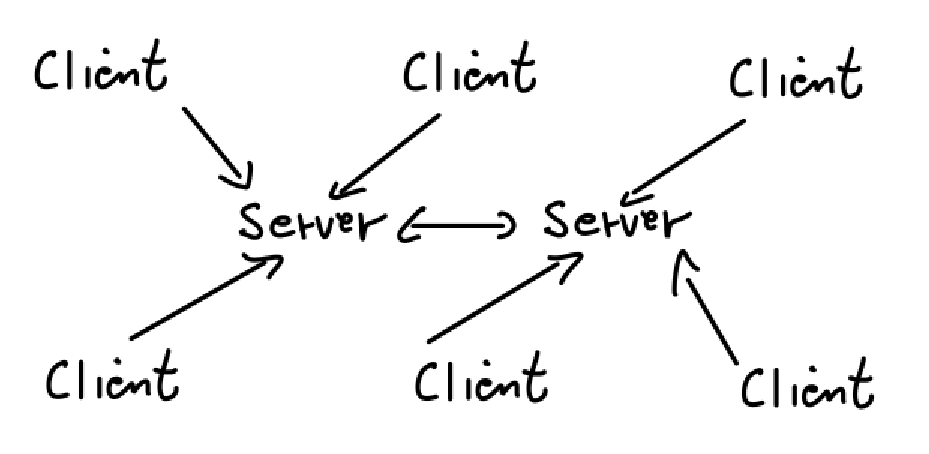
\includegraphics{irc.eps}
\end{figure}
IRC supports 
\textit{direct chat} (one peer to another peer) as well 
as \textit{group chat} (many peers to many peers). The group chat is
realised by creating \textit{IRC channels}, sometimes also called 
\textit{chat rooms}.
% ----------------------------------------------------------------------------
\subsection{Security}
The TLS protocol \cite{rfc2246} is being used in some networks,
but its use is not standardised. Connections from clients to servers
as well as servers to servers may be encrypted.
Some networks support special channel modes to ensure all connected peers
are connected using an encrypted connection. There is no such mode for
direct chat. For normal IRC channels, there is no guarantee that all
peers are connected using an encrypted connection.

Due to its architecture, every operator of a server can listen to all
messages, even if encryption is being used. As the network usually consists
of many clients, but only a small number of servers, an attacker needs
to concentrate on a small number of victim hosts only.
% ----------------------------------------------------------------------------
\section{Secure Internet Live Conferencing (SILC)}
% ----------------------------------------------------------------------------
\subsection{History}
The \textit{ecure Internet Live Conferencing (SILC)} protocol
has been developed by Pekka Riikonen since 1996. The first public release
has been made in 2000. The last releases of SILC software (server and client)
are dated at 2009. Silc can be considered a more secure successor of IRC,
as can be seen in the following quote:
\begin{quote}
[...]
Many of the SILC features are found in traditional chat protocols such 
as IRC but many of the SILC features can also be found in 
Instant Message (IM) style protocols.

SILC combines features from both of these chat protocol styles, 
and can be implemented as either IRC-like system 
or IM-like system.\cite{silcwp}
[...]
\end{quote}

The SILC Project's goal is to fully standardize the SILC protocol in the IETF. 

7 Silc servers

Sep 26, 2009
SILC Server 1.1.18 is out! This version adds heartbeat support and fixes some bugs. 

No version controlled source code, only tar balls from 2009.

Bug form does not return any bugs.
% ----------------------------------------------------------------------------
\subsection{Architecture}
Centralised
% ----------------------------------------------------------------------------
\subsection{Security}
This means that chats might be compromised, if the server itself is compromised. 

SILC Project develops the Secure Internet Live Conferencing protocol (SILC),
\url{http://silcnet.org/general/}

central
\url{http://silcnet.org/support/documentation/wp/silc_protocol.php}

(Ende-zu-Ende-Verschlüsselung).


% ----------------------------------------------------------------------------
\section{XMPP/Jabber}
XMPP, previously named \textit{Jabber}, is the abreviation for
\textit{Extensible Messaging and Presence Protocol}.
It is defined in \cite{rfc3920,rfc3921,rfc3922,rfc3923,rfc4622,rfc4854,rfc4979}
and updated in \cite{rfc6120,rfc6121}.

(XMPP) is an open-standard communications protocol for message-oriented middleware based on XML (Extensible Markup Language).[1] The protocol was originally named Jabber,



% ----------------------------------------------------------------------------
\subsection{History}
Jeremie Miller began working on the Jabber technology in 1998 and released the first version of the jabberd server on January 4, 1999.[5] The early Jabber community focused on open-source software, mainly the jabberd server (e.g., version 1.0 in May 2000, version 1.2 in October 2000, and version 1.4 in February 2001), but its major outcome proved the development of the XMPP protocol.

The XMPP WG produced four specifications (RFC 3920, RFC 3921, RFC 3922, RFC 3923), which were approved by the Internet Engineering Steering Group as Proposed Standards in 2004. The XMPP Standards Foundation (formerly the Jabber Software Foundation) is active in developing open XMPP extensions. In 2011, RFC 3920 and RFC 3921 have been superseded by RFC 6120 and RFC 6121 respectively, and RFC 6122 comes to specify the XMPP address format.

by 2003, was used by over ten million people worldwide, according to the XMPP Standards Foundation.[3]

In February 2010, the social-networking site Facebook opened up its chat feature to third-party applications via XMPP.

% ----------------------------------------------------------------------------
\subsection{Architecture}

Decentralization
The architecture of the XMPP network is similar to email; anyone can run their own XMPP server and there is no central master server.

The XMPP network uses a client–server architecture (clients do not talk directly to one another). 

username@example.com.
% ----------------------------------------------------------------------------
\subsection{Security}
TLS for channel encryption and SASL for authentication

% ----------------------------------------------------------------------------
\section{Skype}
% ----------------------------------------------------------------------------
\subsection{History}
% ----------------------------------------------------------------------------
\subsection{Architecture}
% ----------------------------------------------------------------------------
\subsection{Security}

% ----------------------------------------------------------------------------
\section{Other}
% ----------------------------------------------------------------------------
\subsection{ICQ}
November 1996 veröffentlicht.
 the first Internet-wide instant messaging service, 

America Online acquired Mirabilis on June 8, 1998, for 407dollar million (dollar287 million in cash and dollar120 million over a three-year period based on growth performance levels).

In 2001, ICQ had over 100 million accounts registered.[2] In April 2010, AOL sold ICQ to Digital Sky Technologies for dollar187.5 million.[3]

Uses the oscar \cite{oscar}
Plain text, centralised, auth plaintext or md5 hashed password

% ----------------------------------------------------------------------------
\subsection{MSN}

% ----------------------------------------------------------------------------
\section{Security features and Comparision}

\begin{longtable}{|c|c|c|}
\caption{Chat system comparision with security features}\\
\hline
\textbf{Name} & \textbf{IRC} & \textbf{SILC}\\
\hline
\textbf{Single point of attack} & yes & yes\\
\hline
\textbf{Encrypted traffic} & optional & yes\\
\hline
\end{longtable}

All the solutions with objectives.

\chapter{Analysis of related communication protocols}
% ----------------------------------------------------------------------------
\section{Onion Routing}
% ----------------------------------------------------------------------------
\section{Tor}
% ----------------------------------------------------------------------------
\section{OTR}
\url{http://de.wikipedia.org/wiki/Off-the-Record_Messaging}
% ----------------------------------------------------------------------------
\section{IP}

packet loss: ja
Packet duplicates:
Out of order packets: don't care - no fragmentation
    - probably missing conversation!
    Bit errors: not applicable
    Delay of packets: upper limit (?) 


    - verschieden kaäle:
        - email = sticky, cached, slow
            - tcp = fast, temporarily

            - rudp:
                http://www.javvin.com/protocolRUDP.html
                        rfc908, rfc1151

\subsection{TCP}
Reliable transport
\subsection{UDP}
Connectionless
Reliable connectionless\cite{rfc768}
% ----------------------------------------------------------------------------
\subsection{RUDP}
Reliable connectionless\cite{rfc908,rfc1151}

reliable: (up to a maximum number of retransmissions)
% ----------------------------------------------------------------------------
\section{Enet}

For unreliable packets, ENet will simply discard the lower sequence number packet if a packet with a higher sequence number has already been delivered. This allows the packets to be dispatched immediately as they arrive, and reduce latency of unreliable packets to an absolute minimum. For reliable packets, if a higher sequence number packet arrives, but the preceding packets in the sequence have not yet arrived, ENet will stall delivery of the higher sequence number packets until its predecessors have arrived.


Reliability

ENet provides optional reliability of packet delivery by ensuring the foreign host acknowledges receipt of all reliable packets. ENet will attempt to resend the packet up to a reasonable amount of times, if no acknowledgement of the packet's receipt happens within a specified timeout. Retry timeouts are progressive and become more lenient with every failed attempt to allow for temporary turbulence in network conditions.

Fragmentation and Reassembly

ENet will send and deliver packets regardless of size. Large packets are fragmented into many smaller packets of suitable size, and reassembled on the foreign host to recover the original packet for delivery. The process is entirely transparent to the developer.

Aggregation

ENet aggregates all protocol commands, including acknowledgements and packet transfer, into larger protocol packets to ensure the proper utilization of the connection and to limit the opportunities for packet loss that might otherwise result in further delivery latency.

Adaptability

ENet provides an in-flight data window for reliable packets to ensure connections are not overwhelmed by volumes of packets. It also provides a static bandwidth allocation mechanism to ensure the total volume of packets sent and received to a host don't exceed the host's capabilities. Further, ENet also provides a dynamic throttle that responds to deviations from normal network connections to rectify various types of network congestion by further limiting the volume of packets sent.

Portability

ENet works on Windows and any other Unix or Unix-like platform providing a BSD sockets interface. The library has a small and stable code base that can easily be extended to support other platforms and integrates easily. ENet makes no assumptions about the underlying platform's endianess or word size.

Freedom

ENet demands no royalties and doesn't carry a viral license that would restrict you in how you might use it in your programs. ENet is licensed under a short-and-sweet MIT-style license, which gives you the freedom to do anything you want with it (well, almost anything).

http://enet.bespin.org/

\chapter{Analysis of features and security requirements}
\label{requirements}

\subsection{TO ADD}
From EOF + Latency "`low"', eventual consistency

\subsubsection{Steganographic}
Not for hiding, but to support longer überleben?
http is pretty well suited for this.
mixing with smtp, imap, pop3, tcp. etc.


% -----------------------------------------------------------------------------
From the previous analysis of chat systems and related communication protocols,
several drawbacks can be seen. Most systems suffer a single point of failure,
which is due to the central architecture. Further the message content is often
neither protected nor verified.

The following security features are derived from the weaknesses of the previously
analysed systems as well from the thesis objectives.
% -----------------------------------------------------------------------------
\section{Anonymity}
There are four different types of anonymity:
\begin{itemize}
\item Pseudonymity
\item Sender anonymity
\item Receiver anonymity
\item Sender-receiver anonymity
\end{itemize}
Pseudonymity describes anonymity by using a different identity, for instance
\textit{telmich} instead of Nico Schottelius.
Sender anonymity is present, if nobody can observe who the sender is.
\begin{figure}
    \centering
    \caption[Sender Anonymity]{Sender Anonymity\\Image source: \protect\url{http://www.cs.virginia.edu/crab/anonymity.ppt}}
    \label{senderanon}
    \includegraphics[scale=0.8]{sender-anon.png}
\end{figure}
Receiver anonymity is given, if an observer cannot identify  the receiver of
a message. 
\begin{figure}
    \centering
    \caption[Receiver Anonymity]{Receiver Anonymity\\Image source: \protect\url{http://www.cs.virginia.edu/crab/anonymity.ppt}}
    \label{receiveranon}
    \includegraphics[scale=0.8]{receiver-anon.png}
\end{figure}
If the observer cannot find out whether a given pair of peers
is communicating, Sender-Receiver anonymity is given.
\begin{figure}
    \centering
    \caption[Sender-Receiver Anonymity]{Sender-Receiver Anonymity\\Image source: \protect\url{http://www.cs.virginia.edu/crab/anonymity.ppt}}
    \label{senderreceiveranon}
    \includegraphics[scale=0.8]{sender-receiver-anon.png}
\end{figure}
The three figures \ref{senderanon}, \ref{receiveranon} and
\ref{senderreceiveranon} visualise the differences.
% -----------------------------------------------------------------------------
\subsection{Sender to receiver anonymity}
Providing anonymity of two people talking to each other is \textbf{not} 
required due to the objectives of this thesis.
% Nico: 1 => reformulate
% -----------------------------------------------------------------------------
\subsection{Receiver identification}
The receiver should be able to verify the identity of the sender, so she
can be sure that the message originated from the correct person.
% Nico: 1 => reformulate
% -----------------------------------------------------------------------------
\section{Confidentiality}
The content of the conversations should be hidden from eavesdropper.
Being able to read the content of messages may also reveal the identity
of the chat partners and thus the anonymity would vanish.
% Nico: 1 => reformulate

% FIXME: solution:
% We encrypt every message via public-key cryptography\cite{pgp-1},
% so that only the receiver can decrypt and view the message content.
% 
% -----------------------------------------------------------------------------
\section{Authenticity}

Know who he/she is and that the message is correct.
As messages may contain important content, it is necessary that the integrity
is guaranteed.
% Nico: 1 => reformulate
% -----------------------------------------------------------------------------
\section{Availability}
Most traditional systems rely on central infrastructure to operate, in which a
single party (like the operator) can disable the service. 
No service can be run reliable, if an attacker with infinite resources is assumed.
Thus the requirement for this chat system is to survive the attack of a single
party and to continue delivering the chat service.
% Nico: 1
% -----------------------------------------------------------------------------
%\section{Non security related features}
%To be able to be compete with other chat protocols, \emph{direct} 
%and \emph{group chat} should be supported.
%\subsection{Direct chat
%implemented by two different chat destinations:
%\begin{enumerate}
%\item \emph{Peers}
%\item \emph{Groups of peers}
%\end{enumerate}
%A peer is just another person (direct chat), a group of peers is the EOF
%equivalent of the IRC channel\cite{irc-1}. As there is no central server,
%groups of peers are managed by each client, and thus the compositions of
%group members may be different on different peers.
%-- 
%Additionally, for practical reasons, EOF must support the following
%chat features:
%\begin{enumerate}
%\item Direct chat ("`message is only seen by one person"')
%\item Group chat ("`message is sent to specific group, which may consist of
%more than one person"')
%\end{enumerate}
% -----------------------------------------------------------------------------
\section{Summary}
\begin{enumerate}
%\item Nobody, but the intended receiver(s) know(s) \emph{that} you wrote a message.
\item Nobody, but the intended receiver(s) can view the \emph{message content}.
\item Nobody, but the intended receiver(s) can \emph{verify} the source of the message being you.
\item Nobody, but the intended receiver(s) know(s) \emph{who} the message was sent to.
\item The network must survive attacks of a single attacker.
%\item Hard (if not practilcally impossible) to block chatting.
\end{enumerate}



% ----------------------------------------------------------------------------
\chapter{Chat Protocol Definition}
    4. Protocol definition paper (containing chat features,
            data types, transport methods, security measures)

\subsection{System Design}
The theory behind EOF.
Search for documents proving/supporting the idea.

Different programs handle different objectives
\subsubsection{Use objectives and derive}
\subsubsection{Objective 1 ...}
\subsubsection{Additional constraints}
Cross-OS. Posix and/or ansi-c. ui changable.
\subsubsection{Key Exchange}
Not implemented, manually.
% ----------------------------------------------------------------------------
\subsection{Intra Machine Intra Program Protocol}
\subsubsection{Interfaces}
Sockets, Environment, Paths, etc.
\subsubsection{Data Types}
\subsubsection{Sub Programs}
Consists of the following sub-programs:
encryption, dictionary, key/peer exchange daemon (if possible in this work),
% ----------------------------------------------------------------------------
\subsection{Sub Programs}
Describe what it does, how it does and where it is implemented.
\subsubsection{Noise / Dictionary / Database}
Generate input for times when there is no user input.
Random or db or or or.
Networt traffic
\subsubsection{Encryption}
Splitting of encryption into a seperate program can make use of
multiple computing ressources.
\subsubsection{User Interface}
Own program, indepentend of core.
\subsubsection{Transports}
Receive/Send

% ----------------------------------------------------------------------------
\subsection{Inter Machine Protocol}
On the "`wire"'. Different transports. Constant transport.
Define name (postcard?!) here. Includes transport specific
header / meta information.

\subsubsection{Variable Transports}
Different transports for one peer.
\subsubsection{List of Supported Transports}
To ensure interoperability, clients which support a specific
protocol version must support all listed transport protocols.
\begin{longtable}{|c|c|c|}
\caption{Transport protocols}\\
\hline
\textbf{Protocol} & \textbf{Description} & \textbf{Supported versions}\\
\hline
tcp & Transmission Control Protocol & 0.1 - 0.1\\
\hline
\end{longtable}

\subsubsection{Variable Peers}
Different routes for every packet
\subsubsection{Constant sending}

\subsubsection{Source based routing}
Either here or in Intra Machine Intra Client
\subsubsection{Peer selection}
Which peers, how many. Constant? May give upper bounds of latency.

8 * 0.5seconds = 4 seconds delay.

\subsubsection{Bandwidth usage}
\begin{verbatim}
>>> messages_size=4*1024
>>> messages_per_second=4
>>> bytes_per_second=messages_per_second*messages_size
>>> print(bytes_per_second)
16384
>>> bytes_per_day=86400*bytes_per_second
>>> print(bytes_per_day)
1415577600
>>> print(bytes_per_day/1024**2)
1350.0
>>> bytes_per_month=month_length*bytes_per_day
>>> print(bytes_per_month/1024**2)
41062.5
>>> print(bytes_per_month/1024**3)
40.10009765625
\end{verbatim}
16 KiB/s or 128 KBit/s, 2 ISDN lines. Around 1.4 GiB per day or
circa 40 GiB per month.

% ----------------------------------------------------------------------------
\subsection{Inter Machine Inter Program Protocol}
After decoding the received packet. Forward, etc.
Based on part os EOF simple data types.
\subsubsection{Message types}
List of messages here
\subsubsection{Message 1}
description here

% ----------------------------------------------------------------------------

\section{Basic data types ("`EOFbdt"')}
This section specifies the basic datatypes used in EOF.
% Nico: 1.0
% -----------------------------------------------------------------------------
\subsection{The zero byte}
The zero byte is a byte with the value 0.
% Nico: 1.0
% -----------------------------------------------------------------------------
\subsection{Line feed}
The line feed, "`\textbackslash{}n"', was used to terminate data
sections, but is \emph{DEPRECATED} now.
% Nico: 1.0
% -----------------------------------------------------------------------------
\subsection{ASCII numbers}
ASCII numbers use the decimal string representation of a number (versus
binary representation, which is \emph{never} used between EOFi and EOFs).
ASCII numbers are often used in a packet header.
ASCII numbers are used to specify the length of the packet (excluding itself).
% Nico: 1.0
% -----------------------------------------------------------------------------
\subsection{Strings in general}
Strings are transmitted without termination (i.e. no new line, no 0 byte),
but are padded with zero bytes, if shorter than the specified length.
The encoding to be used is always \textbf{UTF-8}\cite{utf8}.
% Nico: 1.0
% -----------------------------------------------------------------------------
\subsection{Fixed length strings}
Fixed length strings contain exactly the specified number of bytes:
A 128-byte fixed length string consists of at most 128 bytes of text,
which is then not zero terminated!
If the text it contains is shorter than the specified length,
it must be padded with zero bytes.
% Nico: 1.0
% -----------------------------------------------------------------------------
\subsection{Variable length strings}
The EOF protocol currently does not specify any variable length strings.
All strings are fixed length (see above).
% Nico: 1.0
% -----------------------------------------------------------------------------
\subsection{Noise}
There are many situations in which an EOFi sends out data to the network,
although you did not write a message: In fact, as EOFi \textbf{always}
sends packets in a fixed interval, it needs to have data to encrypt and send.

Noise can be any type of random data. As the current random number generators
are quite expensive, it is recommend to use a huge dictionary, old
messages, logfiles, public emails, etc. for noise input.
% Nico: 1.0
% -----------------------------------------------------------------------------
\subsection{Unused}
To make life harder for attackers we try to make packets always be more or
less the same size. That results in fields being present in a packet, which
are unsued.

Unused fields should be filled up with noise.
% Nico: 1.0
% #############################################################################
\section{EOF simple data types ("`EOFsdt"')}
The following sections define the datatypes used in EOF related
applications. The recommened name for use in source
code is added in parentheses after the human understandable name.
% Nico: 1.0
% -----------------------------------------------------------------------------
\subsection{EOF commands and command fields (mapping table)}
An EOF command is exactly \emph{EOF\_L\_CMD} bytes long (fixed length string)
and contains an ASCII number.

EOF commands are the main method of communication between EOFs and EOFi.

The command field 0 indicates the direction.
The command field 1 indicates the EOF subsystem.
\begin{longtable}{|c|c|c|}
\caption{Command fields}\\
\hline
\textbf{Value} & \textbf{Subsystem} / \textbf{Description} & \textbf{Ref}\\
\hline
1*** & Message is coming from the EOF implementation &\\
\hline
10** & \textbf{eofi2tp}: Transport protocols & p\pageref{eofi2tp}\\
\hline
11** & \textbf{eofi2ui}: User interface & p\pageref{eofi2ui}\\
\hline
12** & \textbf{eofi2crypto}: Crypto engine & p\pageref{eofi2crypto}\\
\hline
13** & \textbf{eofi2noise}: Noise generator & p\pageref{eofi2noise}\\
\hline
2*** & Message is coming from EOF subsystem (internally) &\\
\hline
20** & \textbf{eofi2tp}: Transport protocols & p\pageref{eofi2tp}\\
\hline
21** & \textbf{eofi2ui}: User interface & p\pageref{eofi2ui}\\
\hline
22** & \textbf{eofi2crypto}: Crypto engine & p\pageref{eofi2crypto}\\
\hline
23** & \textbf{eofi2noise}: Noise generator & p\pageref{eofi2noise}\\
\hline
3*** & Message is coming from outside ("`onion packet"')) &\\
\hline
\end{longtable}
The command fields 2 and 3 are defined by the respective subsystem.
% -----------------------------------------------------------------------------
\subsection{Identification string (id)}
\label{idn}
To identify a packet, each packet contains an identification string,
which is \emph{EOF\_L\_ID} bytes long. It may contain only the
following characters:
\begin{itemize}
\item A-Z (alphabet in upper case)
\item a-z (alphabet in lower case)
\item 0-9 (the digits)
\item ! (exclamation mark)
\item - (minus)
\end{itemize}
The EOFs or EOFi may chose freely any of the \emph{68719476736}
possibilities.\footnote{$(26+26+10+2)^6$, as long as EOF\_L\_ID is 6.}
The characters are limited to those characters to allow easy debugging
and to keep the non-binary command layout.
% -----------------------------------------------------------------------------
\subsection{Size (size)}
\index{eof.h (File)}%
All sizes used in this document are "`symbolic sizes"': The real size
is defined in the attached file "`\emph{eof.h}"'.
Developers are advised to use the symbolic name in their programs.

A size is is always represented as an ASCII number found in a
fixed length string of \emph{EOF\_L\_SIZE} bytes.
% Nico: 1.0
% -----------------------------------------------------------------------------
\subsection{Nick name (nick)}
The peer name is a \emph{EOF\_L\_NICKNAME} byte fixed length string.
It is only used internally to give a peer a rememberable name ("`a nick'").
It is never transmitted over the network.
% Nico: 1.0
% -----------------------------------------------------------------------------
\subsection{Group name (group)}
The group name is a \emph{EOF\_L\_GROUP} byte fixed length string.
% Nico: 1.0
% -----------------------------------------------------------------------------
\subsection{Message text (msgtext)}
The message text is a \emph{EOF\_L\_MESSAGE} byte fixed length string.
% Nico: 1.0
% -----------------------------------------------------------------------------
\subsection{Peer address (addr)}
The address of a peer, which is is a \emph{EOF\_L\_ADDRESS}
byte fixed length string. Peer addresses are specified as
URLs as defined in RFC3986\cite{uri-1}. For more information have
a look at section \ref{tp} on page \pageref{tp}.
% Nico: 1.0
% -----------------------------------------------------------------------------
\subsection{Keyid, the fingerprint (keyid)}
A (PGP) fingerprint\footnote{See RFC 2440, 11.2. Key IDs and Fingerprints}
is a \emph{EOF\_L\_KEYID} byte fixed length string.
It does not contain any spaces.
It can be retrieved by issuing the following gpg-command:
\begin{verbatim}
LC_ALL=C gpg --fingerprint  | \
   grep "Key fingerprint =" | \
   sed -e 's/.*=//' -e 's/ //g' 
\end{verbatim}
% Nico: 1.0
% #############################################################################
\section{EOF packets ("`EOFpkg"')}
\label{eofpkg}
% -----------------------------------------------------------------------------
\subsection{Introduction}
No packet (including everything) may exceed the size of \emph{EOF\_L\_PKG\_MAX}.

EOF knows about
\begin{itemize}
\item commands: internal plaintext packets.
\item onions: multiple times encrypted packets including routing information
\item postcards: packets containing transport protocol dependent header
\end{itemize}
Commands are the innermost packet type and only seen within EOFi and EOFs.
Commands are then bundled into a multi layer onion. Each layer contains
commands after decryption.
Onions are put onto a postcard afterwards and are sent out on the network.
\textbf{Only encrypted packets are sent out on the network.}
% -----------------------------------------------------------------------------
\subsection{Commands}
Command packets are used for the communication inside of EOFi and EOFs and
are described in detail in the following sections:
\begin{itemize}
\item eofi2tp, \ref{eofi2tp}, page \pageref{eofi2tp}
\item eofi2ui, \ref{eofi2ui}, page \pageref{eofi2ui}
\item eofi2crypto, \ref{eofi2crypto}, page \pageref{eofi2crypto}
\end{itemize}
% Nico: 1.0
% -----------------------------------------------------------------------------
\subsection{Onions}
Onions are sent out on the network and are multiple times encrypted.
They are building the base for the EOF protocol.
Onions are described in detail in chapter \ref{onions}, page \pageref{onions}.
% -----------------------------------------------------------------------------
\subsection{Postcards}
Onions are afterwards encapsulated into the transport protocol specific
packet type and sent out onto the network.
Postcards are described in detail in chapter \ref{postcards}, page \pageref{postcards}.

\section{Basic data types ("`EOFbdt"')}
This section specifies the \textbf{b}asic \textbf{d}ata\textbf{t}ypes. 
They are further referenced as "`EOFbdt"'.
% Nico: 1.0
% -----------------------------------------------------------------------------
\subsection{The zero byte}
The zero byte is a byte with the value 0.
% Nico: 1.0
% -----------------------------------------------------------------------------
\subsection{ASCII numbers}
ASCII numbers use the decimal string representation of a number.
ASCII numbers are often used in a packet header.
ASCII numbers are used to specify the length of the packet (excluding itself).
Due to compatibility of UTF-8 and ASCII, ASCII numbers may also be referred to
as \textit{UTF-8 numbers}.
% Nico: 1.0
% -----------------------------------------------------------------------------
\subsection{Strings in general}
Strings are transmitted without termination (i.e. no new line, no 0 byte).
The encoding to be used is \textbf{UTF-8}\cite{utf8}.
% Nico: 1.0
% -----------------------------------------------------------------------------
\subsection{Fixed length strings}
Fixed length strings contain exactly the specified number of bytes:
A 128-byte fixed length string consists of at most 128 bytes of text.
If the text it contains is shorter than the specified length,
it must be padded with zero bytes.
% Nico: 1.0
% -----------------------------------------------------------------------------
\subsection{Variable length strings}
This protocol does not specify any variable length strings.
% Nico: 1.0

% #############################################################################
\section{EOF simple data types ("`EOFsdt"')}
The following sections define the datatypes used in EOF related
applications. The recommened name for use in source
code is added in parentheses after the human understandable name.
% Nico: 1.0
% -----------------------------------------------------------------------------
\subsection{EOF commands and command fields (mapping table)}
An EOF command is exactly \emph{EOF\_L\_CMD} bytes long (fixed length string)
and contains an ASCII number.

EOF commands are the main method of communication between EOFs and EOFi.

The command field 0 indicates the direction.
The command field 1 indicates the EOF subsystem.
\begin{longtable}{|c|c|c|}
\caption{Command fields}\\
\hline
\textbf{Value} & \textbf{Subsystem} / \textbf{Description} & \textbf{Ref}\\
\hline
1*** & Message is coming from the EOF implementation &\\
\hline
10** & \textbf{eofi2tp}: Transport protocols & p\pageref{eofi2tp}\\
\hline
11** & \textbf{eofi2ui}: User interface & p\pageref{eofi2ui}\\
\hline
12** & \textbf{eofi2crypto}: Crypto engine & p\pageref{eofi2crypto}\\
\hline
13** & \textbf{eofi2noise}: Noise generator & p\pageref{eofi2noise}\\
\hline
2*** & Message is coming from EOF subsystem (internally) &\\
\hline
20** & \textbf{eofi2tp}: Transport protocols & p\pageref{eofi2tp}\\
\hline
21** & \textbf{eofi2ui}: User interface & p\pageref{eofi2ui}\\
\hline
22** & \textbf{eofi2crypto}: Crypto engine & p\pageref{eofi2crypto}\\
\hline
23** & \textbf{eofi2noise}: Noise generator & p\pageref{eofi2noise}\\
\hline
3*** & Message is coming from outside ("`onion packet"')) &\\
\hline
\end{longtable}
The command fields 2 and 3 are defined by the respective subsystem.
% -----------------------------------------------------------------------------
\subsection{Identification string (id)}
\label{idn}
To identify a packet, each packet contains an identification string,
which is \emph{EOF\_L\_ID} bytes long. It may contain only the
following characters:
\begin{itemize}
\item A-Z (alphabet in upper case)
\item a-z (alphabet in lower case)
\item 0-9 (the digits)
\item ! (exclamation mark)
\item - (minus)
\end{itemize}
The EOFs or EOFi may chose freely any of the \emph{68719476736}
possibilities.\footnote{$(26+26+10+2)^6$, as long as EOF\_L\_ID is 6.}
The characters are limited to those characters to allow easy debugging
and to keep the non-binary command layout.
% -----------------------------------------------------------------------------
\subsection{Size (size)}
\index{eof.h (File)}%
All sizes used in this document are "`symbolic sizes"': The real size
is defined in the attached file "`\emph{eof.h}"'.
Developers are advised to use the symbolic name in their programs.

A size is is always represented as an ASCII number found in a
fixed length string of \emph{EOF\_L\_SIZE} bytes.
% Nico: 1.0
% -----------------------------------------------------------------------------
\subsection{Nick name (nick)}
The peer name is a \emph{EOF\_L\_NICKNAME} byte fixed length string.
It is only used internally to give a peer a rememberable name ("`a nick'").
It is never transmitted over the network.
% Nico: 1.0
% -----------------------------------------------------------------------------
\subsection{Group name (group)}
The group name is a \emph{EOF\_L\_GROUP} byte fixed length string.
% Nico: 1.0
% -----------------------------------------------------------------------------
\subsection{Message text (msgtext)}
The message text is a \emph{EOF\_L\_MESSAGE} byte fixed length string.
% Nico: 1.0
% -----------------------------------------------------------------------------
\subsection{Peer address (addr)}
The address of a peer, which is is a \emph{EOF\_L\_ADDRESS}
byte fixed length string. Peer addresses are specified as
URLs as defined in RFC3986\cite{uri-1}. For more information have
a look at section \ref{tp} on page \pageref{tp}.
% Nico: 1.0
% -----------------------------------------------------------------------------
\subsection{Keyid, the fingerprint (keyid)}
A (PGP) fingerprint\footnote{See RFC 2440, 11.2. Key IDs and Fingerprints}
is a \emph{EOF\_L\_KEYID} byte fixed length string.
It does not contain any spaces.
It can be retrieved by issuing the following gpg-command:
\begin{verbatim}
LC_ALL=C gpg --fingerprint  | \
   grep "Key fingerprint =" | \
   sed -e 's/.*=//' -e 's/ //g' 
\end{verbatim}
% Nico: 1.0


\section{EOF packets ("`EOFpkg"')}
\label{eofpkg}
% -----------------------------------------------------------------------------
\subsection{Introduction}
No packet (including everything) may exceed the size of \emph{EOF\_L\_PKG\_MAX}.

EOF knows about
\begin{itemize}
\item commands: internal plaintext packets.
\item onions: multiple times encrypted packets including routing information
\item postcards: packets containing transport protocol dependent header
\end{itemize}
Commands are the innermost packet type and only seen within EOFi and EOFs.
Commands are then bundled into a multi layer onion. Each layer contains
commands after decryption.
Onions are put onto a postcard afterwards and are sent out on the network.
\textbf{Only encrypted packets are sent out on the network.}
% -----------------------------------------------------------------------------
\subsection{Commands}
Command packets are used for the communication inside of EOFi and EOFs and
are described in detail in the following sections:
\begin{itemize}
\item eofi2tp, \ref{eofi2tp}, page \pageref{eofi2tp}
\item eofi2ui, \ref{eofi2ui}, page \pageref{eofi2ui}
\item eofi2crypto, \ref{eofi2crypto}, page \pageref{eofi2crypto}
\end{itemize}
% Nico: 1.0
% -----------------------------------------------------------------------------
\subsection{Onions}
Onions are sent out on the network and are multiple times encrypted.
They are building the base for the EOF protocol.
Onions are described in detail in chapter \ref{onions}, page \pageref{onions}.
% -----------------------------------------------------------------------------
\subsection{Postcards}
Onions are afterwards encapsulated into the transport protocol specific
packet type and sent out onto the network.
Postcards are described in detail in chapter \ref{postcards}, page \pageref{postcards}.


\section{Interface between the chat server and the user interface ("`cs2ui"')}
\label{eofi2ui}
This section specifies how the user interface (UI) communicates with
the chat server (CS).
% Nico: 1.0
% -----------------------------------------------------------------------------
\subsection{Connection}
The chat server provides a TCP listener on port 6667, to which the UI connects 
to. Alternate ports may be used, but need to be specified explicitly.
% -----------------------------------------------------------------------------
\subsection{Messages}
All messages exchanged between CS and the UI are represented as a series
of fixed length strings. Every messages begins with a 
\textbf{command}. Messages send by the chat server use commands
beginning with \textbf{11}, messages send by the
UI use commands that begin with \textbf{21}.
% Nico: ok
% -----------------------------------------------------------------------------
\subsection{Message 1100: Acknowledge}
The is a general acknowledge answer. 
The request with the same \emph{ID} as the packet was successful.
\subsubsection{Parameters}
\begin{longtable}{|c|c|c|c|}
\caption{Command 1100 parameters}\\
\hline
\textbf{Parameter} & \textbf{Type} & \textbf{Description} & \textbf{Example}\\
\hline
ID & EOFsdt: id & packet id & afdb12\\
\hline
\end{longtable}
\subsubsection{Example}
\begin{verbatim}
1100abfudh
\end{verbatim}
% Nico: 2.0
% -----------------------------------------------------------------------------
\subsection{Message 1101: Failure}
The is a general failure answer. The request with the
same \emph{ID} as the packet failed.
Details are specified in the reason message.
\subsubsection{Parameters}
\begin{longtable}{|c|c|c|c|}
\caption{Command 1101 parameters}\\
\hline
\textbf{Parameter} & \textbf{Type} & \textbf{Description} & \textbf{Example}\\
\hline
ID & EOFsdt: id & packet id & afdb12\\
\hline
Reason & EOFsdt: msgtxt & Specifies the failure reason & Too many UIs connected.\\
\hline
\end{longtable}
If the failed command was "`2100"', the CS will close the socket afterwards.
\subsubsection{Example}
\begin{verbatim}
>>> import ceof
>>> ceof.fillup("1101abfudhThe Error Reason", 4+6+256)
'1101abfudhThe Error
Reason\x00\x00\x00\x00\x00\x00\x00\x00\x00\x00\x00\x00\x00\x00\x00\x00\x00\x00
\x00\x00\x00\x00\x00\x00\x00\x00\x00\x00\x00\x00\x00\x00\x00\x00\x00\x00\x00\x00
\x00\x00\x00\x00\x00\x00\x00\x00\x00\x00\x00\x00\x00\x00\x00\x00\x00\x00\x00\x00
\x00\x00\x00\x00\x00\x00\x00\x00\x00\x00\x00\x00\x00\x00\x00\x00\x00\x00\x00\x00
\x00\x00\x00\x00\x00\x00\x00\x00\x00\x00\x00\x00\x00\x00\x00\x00\x00\x00\x00\x00
\x00\x00\x00\x00\x00\x00\x00\x00\x00\x00\x00\x00\x00\x00\x00\x00\x00\x00\x00\x00
\x00\x00\x00\x00\x00\x00\x00\x00\x00\x00\x00\x00\x00\x00\x00\x00\x00\x00\x00\x00
\x00\x00\x00\x00\x00\x00\x00\x00\x00\x00\x00\x00\x00\x00\x00\x00\x00\x00\x00\x00
\x00\x00\x00\x00\x00\x00\x00\x00\x00\x00\x00\x00\x00\x00\x00\x00\x00\x00\x00\x00
\x00\x00\x00\x00\x00\x00\x00\x00\x00\x00\x00\x00\x00\x00\x00\x00\x00\x00\x00\x00
\x00\x00\x00\x00\x00\x00\x00\x00\x00\x00\x00\x00\x00\x00\x00\x00\x00\x00\x00\x00
\x00\x00\x00\x00\x00\x00\x00\x00\x00\x00\x00\x00\x00\x00\x00\x00\x00\x00\x00\x00
\x00\x00'
\end{verbatim}
% Nico: 2.0
% -----------------------------------------------------------------------------
\subsection{Message 1102: Exit requested}
This is a shutdown request to the UI. After this message, the CS will exit.
\subsubsection{Parameters}
\begin{longtable}{|c|c|c|c|}
\caption{Command 1102 parameters}\\
\hline
\textbf{Parameter} & \textbf{Type} & \textbf{Description} & \textbf{Example}\\
\hline
ID & EOFsdt: id & packet id & afdb12\\
\hline
\end{longtable}
\subsubsection{Example}
\begin{verbatim}
1102abf93a
\end{verbatim}
% Nico: 2.0
% -----------------------------------------------------------------------------
\subsection{Message 1103: Received message}
This message is issued by the CS, if a message is received.
\subsubsection{Parameters}
\index{Command!1103}
\begin{longtable}{|c|c|c|c|}
\caption{Command 1103 parameters}\\
\hline
\textbf{Parameter} & \textbf{Type} & \textbf{Description} & \textbf{Example}\\
\hline
ID & EOFsdt: id & packet id & afdb12\\
\hline
name & EOFsdt: name & The sender & telmich\\
\hline
message & EOFsdt: msgtxt & The message & Hallo, mein Freund!\\
\hline
\end{longtable}
\subsubsection{Example}
\begin{verbatim}
>>> import ceof
>>> cmdid="1103abcdef"
>>> name=ceof.fillup("telmich", 128)
>>> message=ceof.fillup("Hallo, mein Freund!", 256)
>>> cmdid + name + message
'1103abcdeftelmich\x00\x00\x00\x00\x00\x00\x00\x00\x00\x00\x00\x00\x00\x00\x00
\x00\x00\x00\x00\x00\x00\x00\x00\x00\x00\x00\x00\x00\x00\x00\x00\x00\x00\x00\x00
\x00\x00\x00\x00\x00\x00\x00\x00\x00\x00\x00\x00\x00\x00\x00\x00\x00\x00\x00\x00
\x00\x00\x00\x00\x00\x00\x00\x00\x00\x00\x00\x00\x00\x00\x00\x00\x00\x00\x00\x00
\x00\x00\x00\x00\x00\x00\x00\x00\x00\x00\x00\x00\x00\x00\x00\x00\x00\x00\x00\x00
\x00\x00\x00\x00\x00\x00\x00\x00\x00\x00\x00\x00\x00\x00\x00\x00\x00\x00\x00\x00
\x00\x00\x00\x00\x00\x00Hallo, mein Freund!\x00\x00\x00\x00\x00\x00\x00\x00\x00
\x00\x00\x00\x00\x00\x00\x00\x00\x00\x00\x00\x00\x00\x00\x00\x00\x00\x00\x00\x00
\x00\x00\x00\x00\x00\x00\x00\x00\x00\x00\x00\x00\x00\x00\x00\x00\x00\x00\x00\x00
\x00\x00\x00\x00\x00\x00\x00\x00\x00\x00\x00\x00\x00\x00\x00\x00\x00\x00\x00\x00
\x00\x00\x00\x00\x00\x00\x00\x00\x00\x00\x00\x00\x00\x00\x00\x00\x00\x00\x00\x00
\x00\x00\x00\x00\x00\x00\x00\x00\x00\x00\x00\x00\x00\x00\x00\x00\x00\x00\x00\x00
\x00\x00\x00\x00\x00\x00\x00\x00\x00\x00\x00\x00\x00\x00\x00\x00\x00\x00\x00\x00
\x00\x00\x00\x00\x00\x00\x00\x00\x00\x00\x00\x00\x00\x00\x00\x00\x00\x00\x00\x00
\x00\x00\x00\x00\x00\x00\x00\x00\x00\x00\x00\x00\x00\x00\x00\x00\x00\x00\x00\x00
\x00\x00\x00\x00\x00\x00\x00\x00\x00\x00\x00\x00\x00\x00\x00\x00\x00\x00\x00\x00
\x00\x00\x00\x00\x00\x00\x00\x00\x00\x00\x00\x00\x00\x00\x00\x00\x00\x00\x00\x00
\x00\x00\x00\x00\x00\x00\x00\x00\x00\x00\x00\x00\x00\x00\x00\x00\x00\x00\x00\x00
\x00\x00\x00\x00\x00\x00\x00\x00'
\end{verbatim}
\subsubsection{Possible answers}
\begin{itemize}
\item None
\end{itemize}
% Nico: 2.0
% -----------------------------------------------------------------------------
\subsection{Message 1104: List of peers}
This is the answer to command \emph{2106}. It contains the same ID, as 
the \emph{2106} request command.
\subsubsection{Parameters}
\begin{longtable}{|c|c|c|c|}
\caption{Command 1104 parameters}\\
\hline
\textbf{Parameter} & \textbf{Type} & \textbf{Description} & \textbf{Example}\\
\hline
ID & EOFsdt: id & packet id & afdb12\\
\hline
Number of peers (nop) & EOFsdt: size & How many peers follow & 20\\
\hline
$nop * Peer$ & EOFsdt: name & The name & telmich\\
\hline
\end{longtable}
The last field is repeated as many times as specified in the number of peers
field.
\subsubsection{Example}
\begin{verbatim}
>>> import ceof
>>> cmd="1104"
>>> eofid = ceof.EOFID()
>>> id = eofid.get_next()
>>> nop=ceof.fillup("2", 6)
>>> peer1=ceof.fillup("telmich", 128)
>>> peer2=ceof.fillup("Hans-Jürgen", 128)
>>> cmd + id + nop + peer1 + peer2
'1104Y7Spet2\x00\x00\x00\x00\x00telmich\x00\x00\x00\x00\x00\x00\x00\x00\x00\x00
\x00\x00\x00\x00\x00\x00\x00\x00\x00\x00\x00\x00\x00\x00\x00\x00\x00\x00\x00\x00
\x00\x00\x00\x00\x00\x00\x00\x00\x00\x00\x00\x00\x00\x00\x00\x00\x00\x00\x00\x00
\x00\x00\x00\x00\x00\x00\x00\x00\x00\x00\x00\x00\x00\x00\x00\x00\x00\x00\x00\x00
\x00\x00\x00\x00\x00\x00\x00\x00\x00\x00\x00\x00\x00\x00\x00\x00\x00\x00\x00\x00
\x00\x00\x00\x00\x00\x00\x00\x00\x00\x00\x00\x00\x00\x00\x00\x00\x00\x00\x00\x00
\x00\x00\x00\x00\x00\x00\x00\x00\x00\x00\x00Hans-Jürgen\x00\x00\x00\x00\x00\x00
\x00\x00\x00\x00\x00\x00\x00\x00\x00\x00\x00\x00\x00\x00\x00\x00\x00\x00\x00\x00
\x00\x00\x00\x00\x00\x00\x00\x00\x00\x00\x00\x00\x00\x00\x00\x00\x00\x00\x00\x00
\x00\x00\x00\x00\x00\x00\x00\x00\x00\x00\x00\x00\x00\x00\x00\x00\x00\x00\x00\x00
\x00\x00\x00\x00\x00\x00\x00\x00\x00\x00\x00\x00\x00\x00\x00\x00\x00\x00\x00\x00
\x00\x00\x00\x00\x00\x00\x00\x00\x00\x00\x00\x00\x00\x00\x00\x00\x00\x00\x00\x00
\x00\x00\x00\x00\x00\x00\x00\x00\x00\x00\x00'
\end{verbatim}
% Nico: 2.0
% -----------------------------------------------------------------------------
\subsection{Message 1105: Peer information}
This is the answer to command \emph{2105}.
It contains the same ID, as the \emph{2105} request command.
\subsubsection{Parameters}
\begin{longtable}{|c|c|c|c|}
\caption{Command 1105 parameters}\\
\hline
\textbf{Parameter} & \textbf{Type} & \textbf{Description} & \textbf{Example}\\
\hline
ID & EOFsdt: id & packet id & afdb12\\
\hline
Keyid & EOFsdt: keyid & This peers pgp-keyid & 389E5481065EAA253...\\
\hline
Number of addresses (noa) & EOFsdt: size & & 2\\
\hline
$noa * address$ & EOFsdt: address & Adress of peer & tcp:127.0.0.1:4243\\
\hline
\end{longtable}
The last field is repeated as often, as specified in the number of addresses
field.
\subsubsection{Example}
\begin{verbatim}
>>> import ceof
>>> cmd="1105"
>>> eofid = ceof.EOFID()
>>> id = eofid.get_next()
>>> keyid="A35767A98CA9CC3CE368679AB679548202C9B17D"
>>> noa=ceof.fillup("2", 6)
>>> addr1=ceof.fillup("tcp://10.2.2.3:4242", 128)
>>> addr2=ceof.fillup("email://nico-eof42@schottelius.org", 128)
>>> cmd + id + keyid + noa + addr1 + addr2
'1105o0mZGMA35767A98CA9CC3CE368679AB679548202C9B17D2\x00\x00\x00\x00\x00
tcp://10.2.2.3:4242\x00\x00\x00\x00\x00\x00\x00\x00\x00\x00\x00\x00\x00\x00\x00
\x00\x00\x00\x00\x00\x00\x00\x00\x00\x00\x00\x00\x00\x00\x00\x00\x00\x00\x00\x00
\x00\x00\x00\x00\x00\x00\x00\x00\x00\x00\x00\x00\x00\x00\x00\x00\x00\x00\x00\x00
\x00\x00\x00\x00\x00\x00\x00\x00\x00\x00\x00\x00\x00\x00\x00\x00\x00\x00\x00\x00
\x00\x00\x00\x00\x00\x00\x00\x00\x00\x00\x00\x00\x00\x00\x00\x00\x00\x00\x00\x00
\x00\x00\x00\x00\x00\x00\x00\x00\x00\x00\x00\x00\x00\x00
email://nico-eof42@schottelius.org\x00\x00\x00\x00\x00\x00\x00\x00\x00\x00\x00
\x00\x00\x00\x00\x00\x00\x00\x00\x00\x00\x00\x00\x00\x00\x00\x00\x00\x00\x00\x00
\x00\x00\x00\x00\x00\x00\x00\x00\x00\x00\x00\x00\x00\x00\x00\x00\x00\x00\x00\x00
\x00\x00\x00\x00\x00\x00\x00\x00\x00\x00\x00\x00\x00\x00\x00\x00\x00\x00\x00\x00
\x00\x00\x00\x00\x00\x00\x00\x00\x00\x00\x00\x00\x00\x00\x00\x00\x00\x00\x00\x00
\x00\x00\x00'
\end{verbatim}
% Nico: 1.0
% -----------------------------------------------------------------------------
\subsection{Message 1106: Peer renamed}
This is the answer to command \emph{2104}. It contains the
same ID, as the \emph{2104} request command.
It is sent out to \textbf{all} connected user interfaces.
\subsubsection{Parameters}
\begin{longtable}{|c|c|c|c|}
\caption{Command 1106 parameters}\\
\hline
\textbf{Parameter} & \textbf{Type} & \textbf{Description} & \textbf{Example}\\
\hline
ID & EOFsdt: id & packet id & afdb12\\
\hline
Old peer name & EOFsdt: name & Old name & susi\\
\hline
New peer name & EOFsdt: name & New name & heinz\\
\hline
\end{longtable}
\subsubsection{Possible answers}
\begin{itemize}
\item None
\end{itemize}
\subsubsection{Example}
\begin{verbatim}
>>> import ceof
>>> cmd="1106"
>>> eofid = ceof.EOFID()
>>> id = eofid.get_next()
>>> oldname=ceof.fillup("telmich", 128)
>>> newname=ceof.fillup("Another Name", 128)
>>> cmd + id + oldname + newname
'1106FpSVy7telmich\x00\x00\x00\x00\x00\x00\x00\x00\x00\x00\x00\x00\x00\x00\x00
\x00\x00\x00\x00\x00\x00\x00\x00\x00\x00\x00\x00\x00\x00\x00\x00\x00\x00\x00\x00
\x00\x00\x00\x00\x00\x00\x00\x00\x00\x00\x00\x00\x00\x00\x00\x00\x00\x00\x00\x00
\x00\x00\x00\x00\x00\x00\x00\x00\x00\x00\x00\x00\x00\x00\x00\x00\x00\x00\x00\x00
\x00\x00\x00\x00\x00\x00\x00\x00\x00\x00\x00\x00\x00\x00\x00\x00\x00\x00\x00\x00
\x00\x00\x00\x00\x00\x00\x00\x00\x00\x00\x00\x00\x00\x00\x00\x00\x00\x00\x00\x00
\x00\x00\x00\x00\x00\x00Another Name\x00\x00\x00\x00\x00\x00\x00\x00\x00\x00\x00
\x00\x00\x00\x00\x00\x00\x00\x00\x00\x00\x00\x00\x00\x00\x00\x00\x00\x00\x00\x00
\x00\x00\x00\x00\x00\x00\x00\x00\x00\x00\x00\x00\x00\x00\x00\x00\x00\x00\x00\x00
\x00\x00\x00\x00\x00\x00\x00\x00\x00\x00\x00\x00\x00\x00\x00\x00\x00\x00\x00\x00
\x00\x00\x00\x00\x00\x00\x00\x00\x00\x00\x00\x00\x00\x00\x00\x00\x00\x00\x00\x00
\x00\x00\x00\x00\x00\x00\x00\x00\x00\x00\x00\x00\x00\x00\x00\x00\x00\x00\x00\x00
\x00\x00\x00\x00\x00'
\end{verbatim}
% Nico: 2.0
% -----------------------------------------------------------------------------
\subsection{Message 2100: Register user interface}
This must be the \emph{first} message sent by the UI. 
If the answer is not \emph{1100}, the UI should close the connection afterwards.
\subsubsection{Parameters}
\begin{longtable}{|c|c|c|c|}
\caption{Command 2100 parameters}\\
\hline
\textbf{Parameter} & \textbf{Type} & \textbf{Description} & \textbf{Example}\\
\hline
ID & EOFsdt: id & packet id & afdb12\\
\hline
Name & EOFsdt: name & Name of the UI & ceofui\\
\hline
\end{longtable}

\subsubsection{Possible answers}
\begin{itemize}
\item 1100
\item 1101
\end{itemize}
\subsubsection{Example}
\begin{verbatim}
>>> import ceof
>>> cmd="2100"
>>> id = ceof.EOFID.int_to_id(42)
>>> name=ceof.fillup("ceofui", 128)
>>> cmd + id + name
'210000000Gceofui\x00\x00\x00\x00\x00\x00\x00\x00\x00\x00\x00\x00\x00\x00\x00
\x00\x00\x00\x00\x00\x00\x00\x00\x00\x00\x00\x00\x00\x00\x00\x00\x00\x00\x00\x00
\x00\x00\x00\x00\x00\x00\x00\x00\x00\x00\x00\x00\x00\x00\x00\x00\x00\x00\x00\x00
\x00\x00\x00\x00\x00\x00\x00\x00\x00\x00\x00\x00\x00\x00\x00\x00\x00\x00\x00\x00
\x00\x00\x00\x00\x00\x00\x00\x00\x00\x00\x00\x00\x00\x00\x00\x00\x00\x00\x00\x00
\x00\x00\x00\x00\x00\x00\x00\x00\x00\x00\x00\x00\x00\x00\x00\x00\x00\x00\x00\x00
\x00\x00\x00\x00\x00\x00\x00'
\end{verbatim}
% Nico: 2.0
% -----------------------------------------------------------------------------
\subsection{Message 2101: Deregister user interface}
\subsubsection{Parameters}
\begin{itemize}
\item none
\end{itemize}
\subsubsection{Possible answers}
\begin{itemize}
\item none
\end{itemize}

The CS will close the connection to the UI after receiving this message.
\subsubsection{Example}
\begin{verbatim}
>>> import ceof
>>> cmd="2101"
>>> cmd
'2101'
\end{verbatim}
% Nico: 2.0
% -----------------------------------------------------------------------------
\subsection{Message 2102: /peer add}
The UI adds a peer to the list of known peers.

\subsubsection{Parameters}
\index{Command!2102: /peer add}%
\begin{longtable}{|c|c|c|c|}
\caption{2102: /peer add parameters}\\
\hline
\textbf{Parameter} & \textbf{Type} & \textbf{Description} & \textbf{Example}\\
\hline
ID & EOFsdt: id & packet id & afdb12\\
\hline
Peer name & EOFsdt: name & Name you identify the peer with & telmich\\
\hline
Address & EOFsdt: addr & Where we can make the first contact & tcp://10.0.42.42:4242\\
\hline
Keyid & EOFsdt: keyid & PGP fingerprint of the peers key & F27987E34E66...\\
\hline
\end{longtable}

\subsubsection{Possible answers}
\begin{itemize}
\item 1100
\item 1101
\end{itemize}
\subsubsection{Example}
\begin{verbatim}
>>> import ceof
>>> cmd="2102"
>>> name=ceof.fillup("telmich", 128)
>>> address=ceof.fillup("tcp://127.0.0.1:6667", 128)
>>> keyid="A35767A98CA9CC3CE368679AB679548202C9B17D"
>>> id = ceof.EOFID.int_to_id(42)
>>> cmd + id + name + address + keyid
'210200000Gtelmich\x00\x00\x00\x00\x00\x00\x00\x00\x00\x00\x00\x00\x00\x00\x00
\x00\x00\x00\x00\x00\x00\x00\x00\x00\x00\x00\x00\x00\x00\x00\x00\x00\x00\x00\x00
\x00\x00\x00\x00\x00\x00\x00\x00\x00\x00\x00\x00\x00\x00\x00\x00\x00\x00\x00\x00
\x00\x00\x00\x00\x00\x00\x00\x00\x00\x00\x00\x00\x00\x00\x00\x00\x00\x00\x00\x00
\x00\x00\x00\x00\x00\x00\x00\x00\x00\x00\x00\x00\x00\x00\x00\x00\x00\x00\x00\x00
\x00\x00\x00\x00\x00\x00\x00\x00\x00\x00\x00\x00\x00\x00\x00\x00\x00\x00\x00\x00
\x00\x00\x00\x00\x00\x00tcp://127.0.0.1:6667\x00\x00\x00\x00\x00\x00\x00\x00\x00
\x00\x00\x00\x00\x00\x00\x00\x00\x00\x00\x00\x00\x00\x00\x00\x00\x00\x00\x00\x00
\x00\x00\x00\x00\x00\x00\x00\x00\x00\x00\x00\x00\x00\x00\x00\x00\x00\x00\x00\x00
\x00\x00\x00\x00\x00\x00\x00\x00\x00\x00\x00\x00\x00\x00\x00\x00\x00\x00\x00\x00
\x00\x00\x00\x00\x00\x00\x00\x00\x00\x00\x00\x00\x00\x00\x00\x00\x00\x00\x00\x00
\x00\x00\x00\x00\x00\x00\x00\x00\x00\x00\x00\x00\x00\x00\x00\x00\x00\x00\x00
A35767A98CA9CC3CE368679AB679548202C9B17D'
\end{verbatim}
% Nico: 1.0
% -----------------------------------------------------------------------------
\subsection{Message 2103: /peer del}
The UI wants to delete a peer.

\subsubsection{Parameters}
\index{Command!/peer del}%
\begin{longtable}{|c|c|c|c|}
\caption{2103: /peer del parameters}\\
\hline
\textbf{Parameter} & \textbf{Type} & \textbf{Description} & \textbf{Example}\\
\hline
ID & EOFsdt: id & packet id & afdb12\\
\hline
Name & EOFsdt: name & Name you identify the peer with & telmich\\
\hline
\end{longtable}

\subsubsection{Possible answers}
\begin{itemize}
\item 1100
\item 1101
\end{itemize}
% Nico: 1.0
\subsubsection{Example}
\begin{verbatim}
>>> import ceof
>>> cmd="2103"
>>> eofid = ceof.EOFID()
>>> id = eofid.get_next()
>>> name=ceof.fillup("telmich", 128)
>>> cmd + id + name
'2103hSJceCtelmich\x00\x00\x00\x00\x00\x00\x00\x00\x00\x00\x00\x00\x00\x00\x00
\x00\x00\x00\x00\x00\x00\x00\x00\x00\x00\x00\x00\x00\x00\x00\x00\x00\x00\x00\x00
\x00\x00\x00\x00\x00\x00\x00\x00\x00\x00\x00\x00\x00\x00\x00\x00\x00\x00\x00\x00
\x00\x00\x00\x00\x00\x00\x00\x00\x00\x00\x00\x00\x00\x00\x00\x00\x00\x00\x00\x00
\x00\x00\x00\x00\x00\x00\x00\x00\x00\x00\x00\x00\x00\x00\x00\x00\x00\x00\x00\x00
\x00\x00\x00\x00\x00\x00\x00\x00\x00\x00\x00\x00\x00\x00\x00\x00\x00\x00\x00\x00
\x00\x00\x00\x00\x00\x00'
\end{verbatim}
% -----------------------------------------------------------------------------
\subsection{Message 2104: /peer rename}
This messages is issued by the UI, when it wants to rename a peer.
\subsubsection{Parameters}
\index{Command!/peer rename}%
\begin{longtable}{|c|c|c|c|}
\caption{/peer rename parameters}\\
\hline
\textbf{Parameter} & \textbf{Type} & \textbf{Description} & \textbf{Example}\\
\hline
ID & EOFsdt: id & packet id & afdb12\\
\hline
Oldnick & EOFsdt: name & Old nick name & susi\\
\hline
Newnick & EOFsdt: name & New nick name & heinz\\
\hline
\end{longtable}

\subsubsection{Possible answers}
\begin{itemize}
\item 1106
\item 1101
\end{itemize}

\subsubsection{Example}
\begin{verbatim}
>>> import ceof
>>> cmd="2104"
>>> eofid = ceof.EOFID()
>>> id = eofid.get_next()
>>> oldname=ceof.fillup("telmich", 128)
>>> newname=ceof.fillup("Another Name", 128)
>>> cmd + id + oldname + newname
'2104zMpcG8telmich\x00\x00\x00\x00\x00\x00\x00\x00\x00\x00\x00\x00\x00\x00\x00
\x00\x00\x00\x00\x00\x00\x00\x00\x00\x00\x00\x00\x00\x00\x00\x00\x00\x00\x00\x00
\x00\x00\x00\x00\x00\x00\x00\x00\x00\x00\x00\x00\x00\x00\x00\x00\x00\x00\x00\x00
\x00\x00\x00\x00\x00\x00\x00\x00\x00\x00\x00\x00\x00\x00\x00\x00\x00\x00\x00\x00
\x00\x00\x00\x00\x00\x00\x00\x00\x00\x00\x00\x00\x00\x00\x00\x00\x00\x00\x00\x00
\x00\x00\x00\x00\x00\x00\x00\x00\x00\x00\x00\x00\x00\x00\x00\x00\x00\x00\x00\x00
\x00\x00\x00\x00\x00\x00Another Name\x00\x00\x00\x00\x00\x00\x00\x00\x00\x00\x00
\x00\x00\x00\x00\x00\x00\x00\x00\x00\x00\x00\x00\x00\x00\x00\x00\x00\x00\x00\x00
\x00\x00\x00\x00\x00\x00\x00\x00\x00\x00\x00\x00\x00\x00\x00\x00\x00\x00\x00\x00
\x00\x00\x00\x00\x00\x00\x00\x00\x00\x00\x00\x00\x00\x00\x00\x00\x00\x00\x00\x00
\x00\x00\x00\x00\x00\x00\x00\x00\x00\x00\x00\x00\x00\x00\x00\x00\x00\x00\x00\x00
\x00\x00\x00\x00\x00\x00\x00\x00\x00\x00\x00\x00\x00\x00\x00\x00\x00\x00\x00\x00
\x00\x00\x00\x00\x00'
\end{verbatim}
% Nico: 2.0
% -----------------------------------------------------------------------------
\subsection{Message 2105: /peer show}
The UI requests details about a peer.

\subsubsection{Parameters}
\begin{longtable}{|c|c|c|c|}
\caption{2105: /peer show parameters}\\
\hline
\textbf{Parameter} & \textbf{Type} & \textbf{Description} & \textbf{Example}\\
\hline
ID & EOFsdt: id & packet id & afdb12\\
\hline
Peer name & EOFsdt: name & Name, as known by the CS & karl-otto\\
\hline
\end{longtable}

\subsubsection{Possible answers}
\begin{itemize}
\item 1101
\item 1105
\end{itemize}
\subsubsection{Example}
\begin{verbatim}
>>> import ceof
>>> cmd="2105"
>>> eofid = ceof.EOFID()
>>> id = eofid.get_next()
>>> name=ceof.fillup("telmich", 128)
>>> cmd  + id + name
'2105wRHWc8telmich\x00\x00\x00\x00\x00\x00\x00\x00\x00\x00\x00\x00\x00\x00\x00
\x00\x00\x00\x00\x00\x00\x00\x00\x00\x00\x00\x00\x00\x00\x00\x00\x00\x00\x00\x00
\x00\x00\x00\x00\x00\x00\x00\x00\x00\x00\x00\x00\x00\x00\x00\x00\x00\x00\x00\x00
\x00\x00\x00\x00\x00\x00\x00\x00\x00\x00\x00\x00\x00\x00\x00\x00\x00\x00\x00\x00
\x00\x00\x00\x00\x00\x00\x00\x00\x00\x00\x00\x00\x00\x00\x00\x00\x00\x00\x00\x00
\x00\x00\x00\x00\x00\x00\x00\x00\x00\x00\x00\x00\x00\x00\x00\x00\x00\x00\x00\x00
\x00\x00\x00\x00\x00\x00'
\end{verbatim}
% Nico: 1.0
% -----------------------------------------------------------------------------
\subsection{Message 2106: /peer list}
The UI requests the list of known peers.

\subsubsection{Parameters}
\begin{longtable}{|c|c|c|c|}
\caption{2106: /peer list parameters}\\
\hline
\textbf{Parameter} & \textbf{Type} & \textbf{Description} & \textbf{Example}\\
\hline
ID & EOFsdt: id & packet id & afdb12\\
\hline
\end{longtable}

\subsubsection{Possible answers}
\begin{itemize}
\item 1101
\item 1104
\end{itemize}
\subsubsection{Example}
\begin{verbatim}
>>> import ceof
>>> cmd="2106"
>>> eofid = ceof.EOFID()
>>> id = eofid.get_next()
>>> cmd + id
'2106LGMsYS'
\end{verbatim}
% Nico: 2.0
% -----------------------------------------------------------------------------
\subsection{Message 2107: /peer send}
The UI wants to submit a message to a peer.

\subsubsection{Parameters}
\index{Command!/peer send}%
\begin{longtable}{|c|c|c|c|}
\caption{2103: /peer send parameters}\\
\hline
\textbf{Parameter} & \textbf{Type} & \textbf{Description} & \textbf{Example}\\
\hline
ID & EOFsdt: id & packet id & afdb12\\
\hline
Peer name & EOFsdt: name & Name you identify the peer with & telmich\\
\hline
Message & EOFsdt: msgtxt & The message itself & Hallo, wie geht es Dir?\\
\hline
\end{longtable}

\subsubsection{Possible answers}
\begin{itemize}
\item 1100
\item 1101
\end{itemize}
\subsubsection{Example}
\begin{verbatim}
>>> import ceof
>>> cmd="2107"
>>> eofid = ceof.EOFID()
>>> id = eofid.get_next()
>>> name=ceof.fillup("telmich", 128)
>>> message=ceof.fillup("Hallo, telmich!", 256)
>>> cmd + id + name + message
'2107NassLAtelmich\x00\x00\x00\x00\x00\x00\x00\x00\x00\x00\x00\x00\x00\x00\x00
\x00\x00\x00\x00\x00\x00\x00\x00\x00\x00\x00\x00\x00\x00\x00\x00\x00\x00\x00\x00
\x00\x00\x00\x00\x00\x00\x00\x00\x00\x00\x00\x00\x00\x00\x00\x00\x00\x00\x00\x00
\x00\x00\x00\x00\x00\x00\x00\x00\x00\x00\x00\x00\x00\x00\x00\x00\x00\x00\x00\x00
\x00\x00\x00\x00\x00\x00\x00\x00\x00\x00\x00\x00\x00\x00\x00\x00\x00\x00\x00\x00
\x00\x00\x00\x00\x00\x00\x00\x00\x00\x00\x00\x00\x00\x00\x00\x00\x00\x00\x00\x00
\x00\x00\x00\x00\x00\x00Hallo, telmich!\x00\x00\x00\x00\x00\x00\x00\x00\x00\x00
\x00\x00\x00\x00\x00\x00\x00\x00\x00\x00\x00\x00\x00\x00\x00\x00\x00\x00\x00\x00
\x00\x00\x00\x00\x00\x00\x00\x00\x00\x00\x00\x00\x00\x00\x00\x00\x00\x00\x00\x00
\x00\x00\x00\x00\x00\x00\x00\x00\x00\x00\x00\x00\x00\x00\x00\x00\x00\x00\x00\x00
\x00\x00\x00\x00\x00\x00\x00\x00\x00\x00\x00\x00\x00\x00\x00\x00\x00\x00\x00\x00
\x00\x00\x00\x00\x00\x00\x00\x00\x00\x00\x00\x00\x00\x00\x00\x00\x00\x00\x00\x00
\x00\x00\x00\x00\x00\x00\x00\x00\x00\x00\x00\x00\x00\x00\x00\x00\x00\x00\x00\x00
\x00\x00\x00\x00\x00\x00\x00\x00\x00\x00\x00\x00\x00\x00\x00\x00\x00\x00\x00\x00
\x00\x00\x00\x00\x00\x00\x00\x00\x00\x00\x00\x00\x00\x00\x00\x00\x00\x00\x00\x00
\x00\x00\x00\x00\x00\x00\x00\x00\x00\x00\x00\x00\x00\x00\x00\x00\x00\x00\x00\x00
\x00\x00\x00\x00\x00\x00\x00\x00\x00\x00\x00\x00\x00\x00\x00\x00\x00\x00\x00\x00
\x00\x00\x00\x00\x00\x00\x00\x00\x00\x00\x00\x00\x00\x00\x00\x00\x00\x00\x00\x00
\x00\x00\x00\x00\x00\x00\x00\x00\x00\x00\x00'
\end{verbatim}
% Nico: 2.0
% -----------------------------------------------------------------------------
\subsection{Message 2199: /quit}
The user interface requests that the CS and all other UIs exit.

\subsubsection{Parameters}
\begin{longtable}{|c|c|c|c|}
\caption{2199: /quit parameters}\\
\hline
\textbf{Parameter} & \textbf{Type} & \textbf{Description} & \textbf{Example}\\
\hline
ID & EOFsdt: id & packet id & afdb12\\
\hline
\end{longtable}

\subsubsection{Possible answers}
\begin{itemize}
\item 1101
\item 1102
\end{itemize}
\subsubsection{Example}
\begin{verbatim}
>>> import ceof
>>> cmd="2199"
>>> eofid = ceof.EOFID()
>>> id = eofid.get_next()
>>> cmd + id
'2199ff5N-j'
\end{verbatim}
% Nico: 2.0

\section{The User Interface ("`ui2user"')}
This section specifies the appereance of the user interface to the user.

% Nico: 1.0
%---------------------------------------------------------------------
\subsection{Interface}
The UI is running as a ncurses application and prompts for input
on a specific line.\footnote{Example output can be found in figure \ref{startup}.}
All commands start with "/".
\begin{figure}
    \caption{UI Startup Screen}
    \label{startup}
    \centering
    \includegraphics[width=10cm]{ui-startup.png}
\end{figure}

%---------------------------------------------------------------------
\subsection{UI Command: /help}
The /help command prints a short usage
description.\footnote{Example output can be found in figure \ref{help}.}

\subsubsection{Example}
\begin{verbatim}
/help
\end{verbatim}
% /connect [host] [port] - Connect to chat server
% /quit - Quit this UI
% /allquit - Quit this UI, Chatserver and all other UIs
% /peer add <name> <address> <keyid> - Add peer
% /peer del <name> - Delete peer
% /peer send <name> <message> - Send message to peer
% /peer rename <oldname> <newname> - Rename peer
% /peer show <name> - Show peer
% /peer list - List all peers
\begin{figure}
    \caption{UI Help Output}
    \label{help}
    \centering
    \includegraphics[width=10cm]{help-command.png}
\end{figure}

%---------------------------------------------------------------------
\subsection{UI Command: /connect $[$host$]$ $[$port$]$}
The connect command can be used to connect to the chat
server.\footnote{Example output can be found in figure \ref{connect}.}
Host and port are optional. If omitted, the saved host and/or
port will be used. This command uses message 2100.
\begin{figure}
    \caption{UI /connect}
    \label{connect}
    \centering
    \includegraphics[width=10cm]{connected-to-cs.png}
\end{figure}

\subsubsection{Example}
\begin{verbatim}
/connect 127.0.0.1 4242
\end{verbatim}
% Nico: Code & Doc
%---------------------------------------------------------------------
\subsection{UI Command: /quit}
Request the user interface to exit. It will deregister from the CS.
This command uses message 2101.
\subsubsection{Example}
\begin{verbatim}
/quit
\end{verbatim}
% Nico: 1.0
%---------------------------------------------------------------------
\subsection{UI Command: /allquit}
The UI tells the CS and all connected UIs (including itself) to quit.
This command uses message 2199.
\begin{figure}
    \caption{UI /allquit}
    \label{allquit}
    \centering
    \includegraphics[width=10cm]{allquit.png}
\end{figure}

\subsubsection{Example}
\begin{verbatim}
/allquit
\end{verbatim}
% Nico: 1.0
%---------------------------------------------------------------------
\subsection{UI Command: /peer add $<$name$>$ $<$address$>$ $<$keyid$>$}
Add the peer with the given name \textit{name} to the list of known peers.

\index{UI Command!/peer add}%
\begin{longtable}{|c|c|c|c|}
\caption{UI Command: /peer add parameters}\\
\hline
\textbf{Parameter} & \textbf{Type} & \textbf{Description} & \textbf{Example}\\
\hline
Peer name & EOFsdt: name & Name you identify the peer with & telmich\\
\hline
Address & EOFsdt: address & Where we can make the first contact & tcp://10.0.42.42:4242\\
\hline
Keyid & EOFsdt: keyid & The PGP fingerprint of the peers public key & F27987E34E66...\\
\hline
\end{longtable}

\subsubsection{Example}
\begin{verbatim}
/peer add telmich tcp//:10.0.42.42:4242 F27987E34E7866B2BA39C2FD793EB8FC325251FE
\end{verbatim}
% Nico: 1.0
%---------------------------------------------------------------------
\subsection{UI Command: /peer del $<$name$>$}
Delete the peer with the given name \textit{name} from the list of known peers.

\index{UI Command!/peer del}%
\begin{longtable}{|c|c|c|c|}
\caption{UI Command: /peer del parameters}\\
\hline
\textbf{Parameter} & \textbf{Type} & \textbf{Description} & \textbf{Example}\\
\hline
Peer name & EOFsdt: name & Name you identify the peer with & telmich\\
\hline
\end{longtable}

\subsubsection{Example}
\begin{verbatim}
/peer del telmich
\end{verbatim}
% Nico: 1.0
%---------------------------------------------------------------------
\subsection{UI Command: /peer send $<$name$>$ $<$msgtext$>$}
Send message \textit{msgtext} to peer \textit{name}.

\index{UI Command!/peer send}%
\begin{longtable}{|c|c|c|c|}
\caption{UI Command: /peer send parameters}\\
\hline
\textbf{Parameter} & \textbf{Type} & \textbf{Description} & \textbf{Example}\\
\hline
Name & EOFsdt: name & Name you identify the peer with & telmich\\
\hline
Msgtext & EOFsdt: msgtxt & The message itself & Hallo, wie geht es Dir?\\
\hline
\end{longtable}

\subsubsection{Example}
\begin{verbatim}
/peer send telmich Hallo, wie geht es Dir?
\end{verbatim}
% Nico: 1.0
%---------------------------------------------------------------------
\subsection{UI Command: /peer rename $<$oldname$>$ $<$newname$>$}
Renames the peer.
\index{UI Command!/peer rename}%
\begin{longtable}{|c|c|c|c|}
\caption{UI Command: /peer rename parameters}\\
\hline
\textbf{Parameter} & \textbf{Type} & \textbf{Description} & \textbf{Example}\\
\hline
Oldname & EOFsdt: name & Old name & susi\\
\hline
Newname & EOFsdt: name & New name & heinz\\
\hline
\end{longtable}

\subsubsection{Example}
\begin{verbatim}
/peer rename susi heinz
\end{verbatim}
% Nico: 1.0
%---------------------------------------------------------------------
\subsection{UI Command: /peer show $<$name$>$}
Display detailled information about peer.
\index{UI Command!/peer show}%
\begin{longtable}{|c|c|c|c|}
\caption{UI Command: /peer rename parameters}\\
\hline
\textbf{Parameter} & \textbf{Type} & \textbf{Description} & \textbf{Example}\\
\hline
Peer name & EOFsdt: name & Name as known by CS & karl-otto\\
\hline
\end{longtable}

\subsubsection{Example}
\begin{verbatim}
/peer show karl-otto
\end{verbatim}
% Nico: 1.0
%---------------------------------------------------------------------
\subsection{UI Command: /peer list}
List of currently known peers. This command does not accept any parameters.

\subsubsection{Example}
\begin{verbatim}
/peer list
\end{verbatim}
% Nico: 1.0
% %---------------------------------------------------------------------
% \subsection{Aliases}
% Aliases may optionally be provided by the UI. If an UI provides
% support for aliases, it must implement the "`\emph{/alias}"' command.
% 
% The following aliases should be provided by default,
% to aid new users using EOF.
% % Nico: 1.0
% %---------------------------------------------------------------------
% \subsection{/alias $<aliasname>$ $<command...>$}
% This command should be used to setup aliases.
% % Nico: 1.0
% %---------------------------------------------------------------------
% \subsection{/msg $<name>$ $<msgtext>$}
% Should be an alias for \textit{/peer send $<$name$>$ $<$msgtext$>$}
% % Nico: 1.0
% %---------------------------------------------------------------------
% \subsection{/whois $<name>$}
% Should be an alias for \textit{/peer show $<$name$>$}
% % Nico: 1.0
\begin{figure}
    \caption{UI /allquit}
    \label{allquit}
    \centering
    \includegraphics[width=10cm]{allquit.png}
\end{figure}

\subsubsection{Example}
\begin{verbatim}
/allquit
\end{verbatim}
% Nico: 1.0
%---------------------------------------------------------------------
\subsection{UI Command: /peer add $<$name$>$ $<$address$>$ $<$keyid$>$}
Add the peer with the given name \textit{name} to the list of known peers.

\index{UI Command!/peer add}%
\begin{longtable}{|c|c|c|c|}
\caption{UI Command: /peer add parameters}\\
\hline
\textbf{Parameter} & \textbf{Type} & \textbf{Description} & \textbf{Example}\\
\hline
Peer name & EOFsdt: name & Name you identify the peer with & telmich\\
\hline
Address & EOFsdt: address & Where we can make the first contact & tcp://10.0.42.42:4242\\
\hline
Keyid & EOFsdt: keyid & The PGP fingerprint of the peers public key & F27987E34E66...\\
\hline
\end{longtable}

\subsubsection{Example}
\begin{verbatim}
/peer add telmich tcp//:10.0.42.42:4242 F27987E34E7866B2BA39C2FD793EB8FC325251FE
\end{verbatim}
% Nico: 1.0
%---------------------------------------------------------------------
\subsection{UI Command: /peer del $<$name$>$}
Delete the peer with the given name \textit{name} form the list of known peers.

\index{UI Command!/peer del}%
\begin{longtable}{|c|c|c|c|}
\caption{UI Command: /peer del parameters}\\
\hline
\textbf{Parameter} & \textbf{Type} & \textbf{Description} & \textbf{Example}\\
\hline
Peer name & EOFsdt: name & Name you identify the peer with & telmich\\
\hline
\end{longtable}

\subsubsection{Example}
\begin{verbatim}
/peer del telmich
\end{verbatim}
% Nico: 1.0
%---------------------------------------------------------------------
\subsection{UI Command: /peer send $<$name$>$ $<$msgtext$>$}
Send message \textit{msgtext} to peer \textit{name}.

\index{UI Command!/peer send}%
\begin{longtable}{|c|c|c|c|}
\caption{UI Command: /peer send parameters}\\
\hline
\textbf{Parameter} & \textbf{Type} & \textbf{Description} & \textbf{Example}\\
\hline
Name & EOFsdt: name & Name you identify the peer with & telmich\\
\hline
Msgtext & EOFsdt: msgtxt & The message itself & Hallo, wie geht es Dir?\\
\hline
\end{longtable}

\subsubsection{Example}
\begin{verbatim}
/peer send telmich Hallo, wie geht es Dir?
\end{verbatim}
% Nico: 1.0
%---------------------------------------------------------------------
\subsection{UI Command: /peer rename $<$oldname$>$ $<$newname$>$}
Renames the peer.
\index{UI Command!/peer rename}%
\begin{longtable}{|c|c|c|c|}
\caption{UI Command: /peer rename parameters}\\
\hline
\textbf{Parameter} & \textbf{Type} & \textbf{Description} & \textbf{Example}\\
\hline
Oldname & EOFsdt & Old name & susi\\
\hline
Newname & EOFsdt & New name & heinz\\
\hline
\end{longtable}

\subsubsection{Example}
\begin{verbatim}
/peer rename susi heinz
\end{verbatim}
% Nico: 1.0
%---------------------------------------------------------------------
\subsection{UI Command: /peer show $<$name$>$}
Display detailled information about peer.
\index{UI Command!/peer show}%
\begin{longtable}{|c|c|c|c|}
\caption{UI Command: /peer rename parameters}\\
\hline
\textbf{Parameter} & \textbf{Type} & \textbf{Description} & \textbf{Example}\\
\hline
Nick name & EOFsdt & Nick name as known by EOFi & karl-otto\\
\hline
\end{longtable}

\subsubsection{Example}
\begin{verbatim}
/peer show karl-otto
\end{verbatim}
% Nico: 1.0
%---------------------------------------------------------------------
\subsection{UI Command: /peer list}
List of currently known peers. This command does not accept any parameters.

\subsubsection{Example}
\begin{verbatim}
/peer list
\end{verbatim}
% Nico: 1.0
% %---------------------------------------------------------------------
% \subsection{Aliases}
% Aliases may optionally be provided by the UI. If an UI provides
% support for aliases, it must implement the "`\emph{/alias}"' command.
% 
% The following aliases should be provided by default,
% to aid new users using EOF.
% % Nico: 1.0
% %---------------------------------------------------------------------
% \subsection{/alias $<aliasname>$ $<command...>$}
% This command should be used to setup aliases.
% % Nico: 1.0
% %---------------------------------------------------------------------
% \subsection{/msg $<name>$ $<msgtext>$}
% Should be an alias for \textit{/peer send $<$name$>$ $<$msgtext$>$}
% % Nico: 1.0
% %---------------------------------------------------------------------
% \subsection{/whois $<name>$}
% Should be an alias for \textit{/peer show $<$name$>$}
% % Nico: 1.0

\section{Noise}
\label{noise}

purpose of ... 

There are many situations in which an EOFi sends out data to the network,
although you did not write a message: In fact, as EOFi \textbf{always}
sends packets in a fixed interval, it needs to have data to encrypt and send.

Noise can be any type of random data. As the current random number generators
are quite expensive, it is recommend to use a huge dictionary, old 
messages, logfiles, public emails, etc. for noise input.
% Nico: 1.0

% ----------------------------------------------------------------------------
\subsection{Fixed interval for sending}
To prevent de-anonymisation by doing statistical analysis on the traffic,
postcards are being at a fixed rate.
In case there is not message to be send, messages with no receiving
party (\textit{noise}) must be used instead.

To avoid problems with different sending intervals
(queuing, buffer exceeding) a network wide fixed sending interval
should be chosen. From the calculations made above, an interval
of \textbf{0.25s} seems to provide a good tradeoff between
latency, anonymity and bandwidth usage.

The number of proxy peers can be choosen by every peer individually
and can be used to focus on smaller bandwidth usage or higher degree
of anonymity. A value of 5 in a network of 100 peers
would make de-anonymising less probable than winning Lotto in Germany
(6 of 49). A value of 8 delays the message at maximum 2 seconds until
it is received.

% ----------------------------------------------------------------------------
\subsection{Latency}
\label{latency}

because every
additional proxy peers adds an amount of time to the latency until the
message arrives.

hoi, hoi ... latency counts afterwards. but includes reaction time.

% ----------------------------------------------------------------------------
\subsubsection{Average Latency}
The average latency for a peer is calculated as follows:
$$\frac{\sum\limits_{i=0}^{(Proxy peers +1)}}{Proxy peers + 1}$$
Depending on how long the waiting delay in seconds is, this results
in different average waiting times for message to arrive, as expressed in
the following formula:
$$Delaytime * \frac{\sum\limits_{i=0}^{(Proxy peers +1)}}{Proxy peers + 1}$$

\begin{longtable}{|c|c|c|c|c|c|c|}
\caption{Average latency based on number of proxy peers}
\label{avglatencypeers}\\
\hline
\multirow{2}{*}{\textbf{Proxy peers}} & \multicolumn{6}{|l|}{\textbf{Average latency (multiplied by delay times)}} \\
& \textbf{(\# timeslots)} & \textbf{0.125s} & \textbf{0.25s} & \textbf{0.5s} & \textbf{1s} & \textbf{2s}\\
\hline
\textbf{1} & 0.5 & 0.0625s & 0.125s & 0.25s & 0.5s & 1s\\
\hline
\textbf{2} & 1 & 0.125s & 0.25s & 0.5s & 1s & 2s\\
\hline
\textbf{3} & 1.5 & 0.1875s & 0.375s & 0.75s & 1.5s & 3s\\
\hline
\textbf{4} & 2 & 0.25s & 0.5s & 1s & 2s & 4s\\
\hline
\textbf{5} & 2.5 & 0.3125s & 0.625s & 1.25s & 2.5s & 5s\\
\hline
\textbf{6} & 3 & 0.375s & 0.75s & 1.5s & 3s & 6s\\
\hline
\textbf{7} & 3.5 & 0.4375s & 0.875s & 1.75s & 3.5s & 7s\\
\hline
\textbf{8} & 4 & 0.5s & 1s & 2s & 4s & 8s\\
\hline
\textbf{9} & 4.5 & 0.5625s & 1.125s & 2.25s & 4.5s & 9s\\
\hline
\textbf{10} & 5 & 0.625s & 1.25s & 2.5s & 5s & 10s\\
\hline
\end{longtable}
A study about 
\textit{System Response Time and User Satisfaction}\cite{responsetime}
indicates that response times up to 6 seconds are tolerable, these numbers
cannot be related directly to the tolerated delay, because the receiving
peer does not know when the sending peer sent a message.
% ----------------------------------------------------------------------------
\subsubsection{Maximum Latency}
Furthermore besides the average latency, the maximum latency needs
to be taken into account, which is shown in table \ref{maxlatencypeers}.
\begin{longtable}{|c|c|c|c|c|c|c|}
\caption{Maximum latency based on number of proxy peers}
\label{maxlatencypeers}\\
\hline
\multirow{2}{*}{\textbf{Proxy peers}} & \multicolumn{6}{|l|}{\textbf{Maximum latency (multiplied by delay times)}} \\
& \textbf{(\# timeslots)} & \textbf{0.125s} & \textbf{0.25s} & \textbf{0.5s} & \textbf{1s} & \textbf{2s}\\
\hline
\textbf{1} & 1 & 0.125s & 0.25s & 0.5s & 1s & 2s\\
\hline
\textbf{2} & 2 & 0.25s & 0.5s & 1s & 2s & 4s\\
\hline
\textbf{3} & 3 & 0.375s & 0.75s & 1.5s & 3s & 6s\\
\hline
\textbf{4} & 4 & 0.5s & 1s & 2s & 4s & 8s\\
\hline
\textbf{5} & 5 & 0.625s & 1.25s & 2.5s & 5s & 10s\\
\hline
\textbf{6} & 6 & 0.75s & 1.5s & 3s & 6s & 12s\\
\hline
\textbf{7} & 7 & 0.875s & 1.75s & 3.5s & 7s & 14s\\
\hline
\textbf{8} & 8 & 1s & 2s & 4s & 8s & 16s\\
\hline
\textbf{9} & 9 & 1.125s & 2.25s & 4.5s & 9s & 18s\\
\hline
\textbf{10} & 10 & 1.25s & 2.5s & 5s & 10s & 20s\\
\hline
\end{longtable}
% ----------------------------------------------------------------------------
\subsection{Bandwidth usage}
Based on the calculated packet sizes (\ref{packetsizes}), 
the following \textbf{outgoing bandwidth}
is needed, as can be seen in table \ref{bandwidth}.
The highest needed bandwidth
in case of 10 proxy peers sending at an interval of 0.125s results in 64 KiB/s
or 512 KBit/s. Todays DSL connections usually exceed this limit by magnitudes
\begin{longtable}{|c|c|c|c|c|c|}
\caption{Outgoing bandwidth usage}
\label{bandwidth}\\
\hline
\multirow{2}{*}{\textbf{Proxy peers}} & \multicolumn{5}{|l|}{\textbf{Intervals / Bandwidth usage in KiB/s}} \\
& \textbf{0.125s} & \textbf{0.25s} & \textbf{0.5s} & \textbf{1s} & \textbf{2s}\\
\hline
\textbf{1} & 9.6 & 4.8 & 2.4 & 1.2 & 0.6\\
\hline
\textbf{2} & 15.2 & 7.6 & 3.8 & 1.9 & 0.95\\
\hline
\textbf{3} & 20.8 & 10.4 & 5.2 & 2.6 & 1.3\\
\hline
\textbf{4} & 26.4 & 13.2 & 6.6 & 3.3 & 1.65\\
\hline
\textbf{5} & 32 & 16 & 8 & 4 & 2\\
\hline
\textbf{6} & 38.4 & 19.2 & 9.6 & 4.8 & 2.4\\
\hline
\textbf{7} & 44.8 & 22.4 & 11.2 & 5.6 & 2.8\\
\hline
\textbf{8} & 50.4 & 25.2 & 12.6 & 6.3 & 3.15\\
\hline
\textbf{9} & 56.8 & 28.4 & 14.2 & 7.1 & 3.55\\
\hline
\textbf{10} & 64 & 32 & 16 & 8 & 4\\
\hline
\end{longtable}
Even on mobile networks, HSUPA Category 1 delivers 0.73 Mbit/s upstream bandwidth.
Older ISDN and Modem connections would not suffice, though
today there are a lot of alternative connections available.\cite{wiki:bitrates}
If using only 9 proxy servers with 0.125s delay or
10 proxy servers with a delay of 0.25s, EDGE could be supported.

The total required network bandwidth is the product of peers in the
network multiplied by the outgoing bandwidth per peer:
$$Required Network Bandwidth = Network Peers * Peer Bandwidth$$
Thus a network with 100 peers, all of them which use 10 proxy peers
and send at a rate of 0.125s, the total required network bandwidth would be
$$RNB = 100 * 64 KiB/s = 6400 KiB/s = 6.25MiB/s = 50 MBit/s$$
If also the receiving side is inside the same network, the required network
bandwith has to be multiplied by two and thus results in 
\textit{100 MBit/s}. This is exactly half of what a fast ethernet switch
can deliver, because fast ethernet provides full duplex 100Mbit/s streams
and thus a single fast ethernet fabric would support 200 simultaneous users.
As the network bandwidth cannot be controlled or influenced by the user
directly, these calculations may simply indicate the network bandwidth
usage for network providers. The user can focus on the bandwith specifications
found in table \ref{bandwidth}.



% -----------------------------------------------------------------------------
\section{EOF messages ("`3***: onions"')}
Onions are the result of decrypting an incoming packet (respective vice versa
when sending out).
% -----------------------------------------------------------------------------
\subsection{Introduction}
The following types are defined:

\begin{itemize}
\item 3000: Drop packet
\item 3001: Forward packet
\item 3002: Message / drop packet
\item 3003: Message / forward packet
\item 3004: Acknowledge
\end{itemize}
% Nico: 1.0
% -----------------------------------------------------------------------------
\subsection{Parameters}
All \textbf{3***} packets have the same length and contain the same fields:
\begin{longtable}{|c|c|c|c|c|}
\caption{Command 3*** parameters}\\
\hline
\textbf{Command} & \textbf{id} & \textbf{addr} & \textbf{group} & \textbf{msgtext}\\
\hline
3000 & - & - & - & - \\
\hline
3001 & - & x & - & - \\
\hline
3002 & x & - & x & x \\
\hline
3003 & x & x & x & x \\
\hline
3004 & x & - & - & -\\
\hline
\end{longtable}

\begin{itemize}
\item -: Not used
\item x: Used
\end{itemize}

\begin{longtable}{|c|c|c|c|}
\caption{Command 3*** parameters}\\
\hline
\textbf{Parameter} & \textbf{Type} & \textbf{Description} & \textbf{Example}\\
\hline
id & EOFsdt & Packet id & alg4f!\\
\hline
addr & EOFsdt & Adress of next peer & tcp:123.123.123.132:8080\\
\hline
group & EOFsdt & The destination group & !eof\\
\hline
msgtext & EOFsdt & The message & Hallo, mein Freund!\\
\hline
\end{longtable}
% Nico: 1.0
% -----------------------------------------------------------------------------
\subsection{3000: Drop packet}
You are the last recipient and there's nothing interesting left.
Just drop the packet and continue work.
% Nico: 1.0
% -----------------------------------------------------------------------------
\subsection{3001: Forward packet}
If a peer receives a packet with the command 3001, it simply forwards
the message to the peer specified in the \textbf{addr} field.
All data contained in the message
is noise. After the message has been forwarded to the next peer, it
should be dropped. If the peer is unreachable, the message should also
be dropped.
% Nico: 1.0
% -----------------------------------------------------------------------------
\subsection{3002: Message / drop packet}
This packet contains a messages to be read and does not need to be forwarded
anymore: You are the last peer in the chain.
\begin{itemize}
\item If the first byte of the group is the zero byte, the message
is a private message (i.e. only sent to you).
\item If the first byte of the group field is \textbf{non-zero} the message
is addressed to the specified group.
\end{itemize}
% Nico: 1.0
% -----------------------------------------------------------------------------
\subsection{3003: Message / forward packet}
The command 3002 is a combination of command 3001 and 3002.
% -----------------------------------------------------------------------------
\subsection{3004: Acknowledge}
Acknowledge the receipt of a received message. The ID must be the same as
the one specified in the original messages packet.
Every message packet must be acknowledged.
% -----------------------------------------------------------------------------
\subsection{Routing}
This version of EOF does not know how to create a route.
All packages are transferred directly to the final peer (which is an
incredible big huge bug) in this version of EOF. Source routing will be
described and defined in future versions.
% Nico: 1.0


% ----------------------------------------------------------------------------
\chapter{Implementation of the Prototype}
% 5. Technical documentation and prototype for the new chat system
% ----------------------------------------------------------------------------
\section{Usage}
How to use.
% ----------------------------------------------------------------------------
\section{Development Process}
spiral
% ----------------------------------------------------------------------------
\section{Environment}
% ----------------------------------------------------------------------------
\subsection{Preperation}
\begin{verbatim}
% virtualenv python-env
% . ./python-env/bin/activate
% pip install python-gnupg
% (cd python-env/bin && ln -s python python3)
\end{verbatim}
python gnupg, virtualenv
Cross-OS. Posix and/or ansi-c. ui changable.
Sockets, Environment, Paths, etc.
Support for different OS would have made development more
hard, so support for POSIX alike operating systems was targeted.

\section{Python and GPG}
Various implementations \cite{python-gpg}
PyMe: 3 Nachrichten in 2010
\url{http://sourceforge.net/mailarchive/forum.php?forum_name=pyme-help&style=threaded}

python-gnupg commits in september 2011 \cite{python-gnupg}

Selected python-gnupg

\subsection{Configuration}
The configuration of EOFi is stored in the cconfig\cite{cconfig} format.
% Nico: FIXME for 1.0: cite

% ----------------------------------------------------------------------------
\section{Related Project: Chat UI}
Own program, indepentend of core, side project
% ----------------------------------------------------------------------------
\section{Code Examples}
% ----------------------------------------------------------------------------
\subsection{Modular Design}
UI seperated.
Portable Core.
id, base 64, 
queuing
forks
manual poll

noise

\subsubsection{Sub Programs}
Consists of the following sub-programs:
encryption, dictionary, key/peer exchange daemon (if possible in this work),
modular design
Different programs handle different objectives

\subsection{Encryption}
Splitting of encryption into a seperate program can make use of
multiple computing ressources.
% ----------------------------------------------------------------------------
\subsection{Noise Engine}
To generate noise, all files from a specific directory are read.
Should be UTF-8 encoded files.

\begin{verbatim}
% cd ~/.ceof 
% mkdir noise
% cd noise 
# Linux Kernel is a good source for noise
% find ~/p/linux/linus -name '*.c' -type f -exec ln -fs {} \;
# Add some rfcs to the noise soup
% find ~/oeffentlich/rechner/netz/rfc/mirror/rfcs-text-only/ -name '*.txt' -type f -exec ln -fs {} \;
% ls | wc -l
23287
\end{verbatim}

Generate input for times when there is no user input.
Random or db or or or.
Networt traffic

\subsection{Transport protocols}
% ----------------------------------------------------------------------------
\section{Command Line Options}

% ----------------------------------------------------------------------------
\section{Tests}
% ----------------------------------------------------------------------------
\subsection{Performance}
%\subsection{Packet size}
Re-testing of crypt (using test/recrypt): 5.2 - 5.3 KiB per packet.

\subsection{Bandwidth usage}
After protocol overhead...

% ----------------------------------------------------------------------------


% ----------------------------------------------------------------------------
\section{Supported Features}
Based on the requirements defined in \ref{requirements}, 
p. \pageref{requirements}, the following features have been implemented. 
% MIRROR of that chapter here!

% ----------------------------------------------------------------------------
\subsection{Anonymity}
Multi-Hop onion routingg

Sender verification
Before the encrypt the packet, it is signed via public-key
cryptography\cite{pgp-1}. Thus only the receiver can verify the message sender.

\subsubsection{obfuscation}
- Hide message sending 

We don't think it's possible to hide that you are part of the chat network,
because some heuristics will be developed to detect the chat packets.
So we use a different idea:
Every participant of an EOF network will constantly send chat packets
with a pre-defined frequency (for instance every 250 ms). 
If you don't chat, \emph{noise} is sent.\footnote{Noise is just random
data, see below for a more detailled description of noise.}
The noise is also used to defend against timing analysis.
In case you are sending out a message, the message packet will be added to the
queue and sent within the next free time slot.

From outside it can easily be seen, that you are part of the network,
but not, if you sent a message.

\subsubsection{Hide message receiver}
The message packets are always sent indirectly via onion routing\cite{onion-1}.
The idea is taken from the Tor project\cite{tor-1}, though EOF uses an enhanced
version: EOF does not know about entry or exit nodes. If you are the intended
receiver you may or may not continue to forward the message, which is defined
by the sender of the message. That said, EOF must use source 
routing\cite{source-routing-1}.

To support onion routing, the sender of a packet needs to encrypt the packet
multiple times, once for each host that receives the packet. This may look
as follows:
\begin{enumerate}
\item Create message (from noise or user input)
\item Create source path
\item Create packet for last peer ("`pkg-last"')
\item Create packet for last-1 peer including \emph{pkg-last}
\item Continue until first peer is reached
\item Sent packet to first peer 
\end{enumerate}
Thus every peer only knows the previous and the next peer.
% Nico: 1.0


\subsection{Availability}
To prevent
successful elimination of the service, a decentralised architecture should


\subsubsection{Reliable against single user attacks}
Traditional chat networks depend on one or more central organised servers.
An attacker can stop all communication, if she runs a successful denial
of service ("`DoS"') attack against the central systems.
To protect against this, EOF uses a dynamic peer-to-peer network, which works
as long as the minimun number of peers and the destination peer is available.
It has no dependency on a central server.

\subsubsection{Hide packets in network stream}
As said before, we don't think it's possible to hide the participation in the
chat network. To be able to send packets, although an attacker \emph{knows}
about the participation, EOF embeds all chat packets into other (well known)
protocols (which is knows as steganography\cite{stegano-1}).
EOF does not implement nor specify \emph{transport protocols} itself.
The EOF community is urged to implement them in a creative way: Usage
of well-known protocols like TCP\cite{tcp-1}, HTTP\cite{http-1},
SMTP\cite{smtp-1} or even transmission of packets on avian
carriers\cite{avian-1} are encouraged. The tunneling of EOF packets through
those protocols (also know as obfuscation) makes it harder to detect
and \emph{block} EOF traffic. 
If an attacker wants you to stop sending messages, she has to completly
remove you from the network, because any open protocol may be (ab)used to
encapsulate EOF packets into it.
% Nico: 1.0 




\subsection{Confidentiality}

\subsection{Integrity}
Before the encrypt the packet, it is signed via public-key
cryptography\cite{pgp-1}. Thus only the receiver can verify the message sender.


% ----------------------------------------------------------------------------
\section{Usage}


% #############################################################################
\section{Transport protocols ("`eofi2tp"')}
\label{eofi2tp}
% -----------------------------------------------------------------------------
\subsection{Definition/Specification}
URL, URI, Scheme clearification, use tcp:// and http:// syntax.


% -----------------------------------------------------------------------------
\subsection{Introduction}
Every transport protocol consists of a listening (\verb=listen=)
and sending (\verb=send=) part. When the EOFi starts, it starts all
transport protocols, which should the remain started and listen
for commands issued by the EOFi.
URLs are used as defined in RFC3986\cite{uri-1}.
For schemes only lower-case names are allowed
(to prevent problems with case-insensitive filesystems).
% -----------------------------------------------------------------------------
\subsection{Paths}
\label{tppaths}
All paths are relative to the directory p\_tp\_d, as described
in \ref{ptpd} on p. \pageref{ptpd}.
\begin{longtable}{|c|c|}
\caption{Required transport protocols}\\
\hline
\textbf{Scheme} & \textbf{Name}\\
\hline
\verb=available/= & Available transport procols\\
\hline
\verb=available/<scheme>/listen= & Listener (executable) for the scheme\\
\hline
\verb=available/<scheme>/send= & Sender (executable) for the scheme\\
\hline
\verb=listen/= & Enabled listeners\\
\hline
\verb=listen/<freeform>/url= & URL \\
\hline
\end{longtable}
% -----------------------------------------------------------------------------
\subsubsection{Enabling a scheme}
\label{tpscheme}
To enable support for the scheme \verb=http=
create both, the \verb=listen= and the \verb=send= executable below
\verb=available/http=.
% Nico: 1.0
% -----------------------------------------------------------------------------
\subsubsection{Enabling a listener}
\label{tplisten}
To enable a listener for the scheme \emph{http} at the URL
\emph{http://www.example.com/eof}, create
the directory \verb=listen/http-example= and the file
\verb=listen/http-example/url= with the content
\verb=http://www.example.com/eof=.
If the transport protocol implementation needs or allows additional
configuration files, they should be placed in the same directory.
The EOF implementation will parse the URL and check whether the
scheme is supported.
% Nico: 1.0
% -----------------------------------------------------------------------------
\subsection{Required implementations}
\label{tprequired}
This version of the EOF standard requires support for the following
transport protocols in the implementation:
\begin{longtable}{|c|c|c|c|}
\caption{Required transport protocols}\\
\hline
\textbf{Scheme} & \textbf{Name} & \textbf{Format} & \textbf{Description}\\
\hline
tcp & IP/TCP & \verb=tcp:host:port= & Plain tcp\\
\hline
\end{longtable}
% -----------------------------------------------------------------------------
\subsection{Upcoming implementations}
\label{tpupcoming}
The following transport protocol implementations have been proposed,
but are not yet implemented and thus not yet part of the standard:

\begin{longtable}{|c|c|c|c|}
\caption{Upcoming transport protocols}\\
\hline
\textbf{Scheme} & \textbf{Name} & \textbf{Format} & \textbf{Description}\\
\hline
dns & DNS       & \verb=dns:host:port:type= & Package via DNS\\
\hline
http & HTTP       & \verb=http:host:port/path= & Plain http\\
\hline
https & HTTPS     & \verb=https:host:port/path= & http with ssl\\
\hline
mailto & E-Mail   & \verb=mailo:address= & Send package as e-mail\\
\hline
mediawiki & Mediawiki   & \verb=mediawiki:host:port:page= & Transfer via Mediawiki\\
\hline
smb  & SMB     & \verb=smb:[user[:password]@]host:path= & Server message block\\
\hline
smtp & SMTP     & \verb=smtp:[user[:password]@]host:port= & http with ssl\\
\hline
tcps & IP/TCP/SSL & \verb=tcps:host:port= & tcp with ssl around\\
\hline
udp & IP/UPD      & \verb=udp:host:port= & Plain UDP\\
\hline
\end{longtable}
% -----------------------------------------------------------------------------
\subsection{Developing and integrating implementations}
If you want to create a new transport protocol, create the two
executables as described in \ref{tppaths} and put them in their
scheme directory.
If the implementation works fine and you would like to add it to EOF,
create the directory \verb=tp/<scheme>/<implementation_name>= within
the EOFi source directory and update the following
sections of this document:
\begin{itemize}
\item \ref{tprequired}
\item \ref{tprequired} / new subsubsection for the new scheme
\item \ref{tpupcoming}
\end{itemize}

The name of the subsubsection is the name of the scheme
plus the registered implementation ("`like tcp-c"').
Every such subsubsection must at least contain:
\begin{itemize}
\item Author contact information
\item URL of website
\item Programming language
\end{itemize}
Keep the subsubsections sorted by alphabet.
% Nico: 1.0
% -----------------------------------------------------------------------------
\subsection{1000: Send packet}
\index{Command!1000}
\begin{longtable}{|c|c|c|c|}
\caption{Command 1000 parameters}\\
\hline
\textbf{Parameter} & \textbf{Type} & \textbf{Description} & \textbf{Example}\\
\hline
ID & EOFsdt: id & packet id & afdb12\\
\hline
Destination & EOFsdt: addr & complete URL (with "`\emph{scheme:}"') & tcp:127.0.0.3:42\\
\hline
Size & EOFsdt: size & Size of message, excluding this header & 424242\\
\hline
Message & Binary data & The message & BLOB\\
\hline
\end{longtable}
\subsubsection{Possible answers}
\begin{itemize}
\item 2000
\item 2001
\end{itemize}
% -----------------------------------------------------------------------------
\subsubsection{1000: Example}
Added linebreak after some \textbackslash{}0 for readability, which are \textbf{not} in
the real packet!
\begin{verbatim}
1000abfudh127.0.0.3:42\0\0\0\0\0\0\0\0\0\0\0\0\0\0\0\0\0\0\0\0\0\0\0\0\0\0\0\0
\0\0\0\0\0\0\0\0\0\0\0\0\0\0\0\0\0\0\0\0\0\0\0\0\0\0\0\0\0\0\0\0\0\0\0\0\0\0\0
\0\0\0\0\0\0\0\0\0\0\0\0\0\0\0\0\0\0\0\0\0\0\0\0\0\0\0\0\0\0\0\0\0\0\0\0\0\0\0
\0\0\0\0\0\0\0\0\0\010\0\0\0\0HEREISDATA
\end{verbatim}
% Nico: 1.0
% -----------------------------------------------------------------------------
\subsection{1001: Enable listening}
\index{Command!1001}%
When the listening transport protocol starts up, EOFi sends this command and
waits for the acknowledge package, before it marks the transport protocol as enabled.
\begin{longtable}{|c|c|c|c|}
\caption{Command 1001 parameters}\\
\hline
\textbf{Parameter} & \textbf{Type} & \textbf{Description} & \textbf{Example}\\
\hline
ID & EOFsdt: id & packet id & afdb12\\
\hline
Destination & EOFsdt: addr & URL without "`\emph{scheme:}"' & 127.0.0.3:42\\
\hline
\end{longtable}
\subsubsection{Possible answers}
\begin{itemize}
\item 2003
\end{itemize}
% -----------------------------------------------------------------------------
\subsubsection{1001: Example}
\begin{verbatim}
1001afdb12127.0.0.3:42\0\0\0\0\0\0\0\0\0\0\0\0\0\0\0\0\0\0\0\0\0\0\0\0\0
\0\0\0\0\0\0\0\0\0\0\0\0\0\0\0\0\0\0\0\0\0\0\0\0\0\0\0\0\0\0\0\0\0\0\0\0
\0\0\0\0\0\0\0\0\0\0\0\0\0\0\0\0\0\0\0\0\0\0\0\0\0\0\0\0\0\0\0\0\0\0\0\0
\0\0\0\0\0\0\0\0\0\0\0\0\0\0\0\0\0\0\0
\end{verbatim}
% -----------------------------------------------------------------------------
\subsection{1002: Stop listening}
\index{Command!1002}%
This command requests a listening transport protocol to shutdown.
It should free all ressources and exit. After a grace time (maybe seconds,
not yet defined), EOFi will kill the badly behaving transport protocol.
\begin{longtable}{|c|c|c|c|}
\caption{Command 1001 parameters}\\
\hline
\textbf{Parameter} & \textbf{Type} & \textbf{Description} & \textbf{Example}\\
\hline
ID & EOFsdt: id & packet id & afdb12\\
\hline
\end{longtable}
\subsubsection{Possible answers}
\begin{itemize}
\item none
\end{itemize}
% -----------------------------------------------------------------------------
\subsection{1003: Prepare sending}
\index{Command!1003}%
This command requests a transport protocol sender to prepare for sending out
data. The transport protocol should initialise itself and acknowledge
when it is ready for sending.
\begin{longtable}{|c|c|c|c|}
\caption{Command 1003 parameters}\\
\hline
\textbf{Parameter} & \textbf{Type} & \textbf{Description} & \textbf{Example}\\
\hline
ID & EOFsdt: id & packet id & afdb12\\
\hline
\end{longtable}
\subsubsection{Possible answers}
\begin{itemize}
\item none
\end{itemize}
% -----------------------------------------------------------------------------
\subsection{1004: Stop sending}
\index{Command!1004}%
This command requests a transport protocol sender to shutdown.
It should free all ressources and exit. After a grace time (maybe seconds,
not yet defined), EOFi will kill the badly behaving transport protocol.
\begin{longtable}{|c|c|c|c|}
\caption{Command 1004 parameters}\\
\hline
\textbf{Parameter} & \textbf{Type} & \textbf{Description} & \textbf{Example}\\
\hline
ID & EOFsdt: id & packet id & afdb12\\
\hline
\end{longtable}
\subsubsection{Possible answers}
\begin{itemize}
\item none
\end{itemize}
% -----------------------------------------------------------------------------
\subsection{2000: Packet successfully sent}
This code is returned by the transport protocol subsystem to EOFi on success.
After this return code, the transport protocol exits.
\begin{longtable}{|c|c|c|c|}
\caption{Command 2000 parameters}\\
\hline
\textbf{Parameter} & \textbf{Type} & \textbf{Description} & \textbf{Example}\\
\hline
ID & EOFsdt: id & packet id & afdb12\\
\hline
\end{longtable}
\subsubsection{Possible answers}
\begin{itemize}
\item none
\end{itemize}
% -----------------------------------------------------------------------------
\subsection{2001: Packet not sent}
\index{Command!2001}
This code is returned by the transport protocol subsystem to the
EOF implementation on failure.
After this return code, the transport protocol exits.
\begin{longtable}{|c|c|c|c|}
\caption{Command 2001 parameters}\\
\hline
\textbf{Parameter} & \textbf{Type} & \textbf{Description} & \textbf{Example}\\
\hline
ID & EOFsdt: id & packet id & afdb12\\
\hline
\end{longtable}
\subsubsection{Possible answers}
\begin{itemize}
\item none
\end{itemize}
% -----------------------------------------------------------------------------
\subsection{2002: Received packet}
\index{Command!2002}
The listening transport protocol received a packet and notifies EOFi.
\begin{longtable}{|c|c|c|c|}
\caption{Command 2002 parameters}\\
\hline
\textbf{Parameter} & \textbf{Type} & \textbf{Description} & \textbf{Example}\\
\hline
ID & EOFsdt: id & packet id & afdb12\\
\hline
Size & EOFsdt:size & Excluding the 2002 and this field & 42\\
\hline
Message & Binary data & The message & BLOB\\
\hline
\end{longtable}
\subsubsection{Possible answers}
\begin{itemize}
\item none
\end{itemize}
% -----------------------------------------------------------------------------
\subsection{2003: Listening}
\index{Command!2003}
This code is returned by the listening transport protocol, as soon as the
listening process is ready to receive data. After that, EOFi can announce
the listening URL to other EOFi.
\begin{longtable}{|c|c|c|c|}
\caption{Command 2003 parameters}\\
\hline
\textbf{Parameter} & \textbf{Type} & \textbf{Description} & \textbf{Example}\\
\hline
ID & EOFsdt: id & packet id & afdb12\\
\hline
\end{longtable}
\subsubsection{Possible answers}
\begin{itemize}
\item none
\end{itemize}
% -----------------------------------------------------------------------------
\subsection{2004: Not listening}
\index{Command!2004}
If something happended that makes the listening transport protocol
unable to startup, it issues this command and exits afterwards.
\begin{longtable}{|c|c|c|c|}
\caption{Command 2004 parameters}\\
\hline
\textbf{Parameter} & \textbf{Type} & \textbf{Description} & \textbf{Example}\\
\hline
ID & EOFsdt: id & packet id & afdb12\\
\hline
Reason & EOFsdt: msgtxt & Why the connection was refused & Too many UIs connected.\\
\hline
\end{longtable}
\subsubsection{Possible answers}
\begin{itemize}
\item none
\end{itemize}
% -----------------------------------------------------------------------------
\subsection{2005: Ready for sending}
\index{Command!2005}
This code is returned by the transport protocol sender, as soon as the
process is ready to send data.
\begin{longtable}{|c|c|c|c|}
\caption{Command 2005 parameters}\\
\hline
\textbf{Parameter} & \textbf{Type} & \textbf{Description} & \textbf{Example}\\
\hline
ID & EOFsdt: id & packet id & afdb12\\
\hline
\end{longtable}
\subsubsection{Possible answers}
\begin{itemize}
\item none
\end{itemize}
% -----------------------------------------------------------------------------
\subsection{2006: Sender preperation error}
\index{Command!2006}
If something happended that makes the transport protocol sender
unable to startup, it issues this command and exits afterwards.
\begin{longtable}{|c|c|c|c|}
\caption{Command 2006 parameters}\\
\hline
\textbf{Parameter} & \textbf{Type} & \textbf{Description} & \textbf{Example}\\
\hline
ID & EOFsdt: id & packet id & afdb12\\
\hline
Reason & EOFsdt: msgtxt & Why the connection was refused & Too many UIs connected.\\
\hline
\end{longtable}
\subsubsection{Possible answers}
\begin{itemize}
\item none
\end{itemize}
% #############################################################################
% #############################################################################



% #############################################################################
\section{Transport protocols ("`eofi2tp"')}
\label{eofi2tp}
% -----------------------------------------------------------------------------
\subsection{Definition/Specification}
URL, URI, Scheme clearification, use tcp:// and http:// syntax.


% -----------------------------------------------------------------------------
\subsection{Introduction}
Every transport protocol consists of a listening (\verb=listen=)
and sending (\verb=send=) part. When the EOFi starts, it starts all
transport protocols, which should the remain started and listen
for commands issued by the EOFi.
URLs are used as defined in RFC3986\cite{uri-1}.
For schemes only lower-case names are allowed
(to prevent problems with case-insensitive filesystems).
% -----------------------------------------------------------------------------
\subsection{Paths}
\label{tppaths}
All paths are relative to the directory p\_tp\_d, as described
in \ref{ptpd} on p. \pageref{ptpd}.
\begin{longtable}{|c|c|}
\caption{Required transport protocols}\\
\hline
\textbf{Scheme} & \textbf{Name}\\
\hline
\verb=available/= & Available transport procols\\
\hline
\verb=available/<scheme>/listen= & Listener (executable) for the scheme\\
\hline
\verb=available/<scheme>/send= & Sender (executable) for the scheme\\
\hline
\verb=listen/= & Enabled listeners\\
\hline
\verb=listen/<freeform>/url= & URL \\
\hline
\end{longtable}
% -----------------------------------------------------------------------------
\subsubsection{Enabling a scheme}
\label{tpscheme}
To enable support for the scheme \verb=http=
create both, the \verb=listen= and the \verb=send= executable below
\verb=available/http=.
% Nico: 1.0
% -----------------------------------------------------------------------------
\subsubsection{Enabling a listener}
\label{tplisten}
To enable a listener for the scheme \emph{http} at the URL
\emph{http://www.example.com/eof}, create
the directory \verb=listen/http-example= and the file
\verb=listen/http-example/url= with the content
\verb=http://www.example.com/eof=.
If the transport protocol implementation needs or allows additional
configuration files, they should be placed in the same directory.
The EOF implementation will parse the URL and check whether the
scheme is supported.
% Nico: 1.0
% -----------------------------------------------------------------------------
\subsection{Required implementations}
\label{tprequired}
This version of the EOF standard requires support for the following
transport protocols in the implementation:
\begin{longtable}{|c|c|c|c|}
\caption{Required transport protocols}\\
\hline
\textbf{Scheme} & \textbf{Name} & \textbf{Format} & \textbf{Description}\\
\hline
tcp & IP/TCP & \verb=tcp:host:port= & Plain tcp\\
\hline
\end{longtable}
% -----------------------------------------------------------------------------
\subsection{Upcoming implementations}
\label{tpupcoming}
The following transport protocol implementations have been proposed,
but are not yet implemented and thus not yet part of the standard:

\begin{longtable}{|c|c|c|c|}
\caption{Upcoming transport protocols}\\
\hline
\textbf{Scheme} & \textbf{Name} & \textbf{Format} & \textbf{Description}\\
\hline
dns & DNS       & \verb=dns:host:port:type= & Package via DNS\\
\hline
http & HTTP       & \verb=http:host:port/path= & Plain http\\
\hline
https & HTTPS     & \verb=https:host:port/path= & http with ssl\\
\hline
mailto & E-Mail   & \verb=mailo:address= & Send package as e-mail\\
\hline
mediawiki & Mediawiki   & \verb=mediawiki:host:port:page= & Transfer via Mediawiki\\
\hline
smb  & SMB     & \verb=smb:[user[:password]@]host:path= & Server message block\\
\hline
smtp & SMTP     & \verb=smtp:[user[:password]@]host:port= & http with ssl\\
\hline
tcps & IP/TCP/SSL & \verb=tcps:host:port= & tcp with ssl around\\
\hline
udp & IP/UPD      & \verb=udp:host:port= & Plain UDP\\
\hline
\end{longtable}
% -----------------------------------------------------------------------------
\subsection{Developing and integrating implementations}
If you want to create a new transport protocol, create the two
executables as described in \ref{tppaths} and put them in their
scheme directory.
If the implementation works fine and you would like to add it to EOF,
create the directory \verb=tp/<scheme>/<implementation_name>= within
the EOFi source directory and update the following
sections of this document:
\begin{itemize}
\item \ref{tprequired}
\item \ref{tprequired} / new subsubsection for the new scheme
\item \ref{tpupcoming}
\end{itemize}

The name of the subsubsection is the name of the scheme
plus the registered implementation ("`like tcp-c"').
Every such subsubsection must at least contain:
\begin{itemize}
\item Author contact information
\item URL of website
\item Programming language
\end{itemize}
Keep the subsubsections sorted by alphabet.
% Nico: 1.0
% -----------------------------------------------------------------------------
\subsection{1000: Send packet}
\index{Command!1000}
\begin{longtable}{|c|c|c|c|}
\caption{Command 1000 parameters}\\
\hline
\textbf{Parameter} & \textbf{Type} & \textbf{Description} & \textbf{Example}\\
\hline
ID & EOFsdt: id & packet id & afdb12\\
\hline
Destination & EOFsdt: addr & complete URL (with "`\emph{scheme:}"') & tcp:127.0.0.3:42\\
\hline
Size & EOFsdt: size & Size of message, excluding this header & 424242\\
\hline
Message & Binary data & The message & BLOB\\
\hline
\end{longtable}
\subsubsection{Possible answers}
\begin{itemize}
\item 2000
\item 2001
\end{itemize}
% -----------------------------------------------------------------------------
\subsubsection{1000: Example}
Added linebreak after some \textbackslash{}0 for readability, which are \textbf{not} in
the real packet!
\begin{verbatim}
1000abfudh127.0.0.3:42\0\0\0\0\0\0\0\0\0\0\0\0\0\0\0\0\0\0\0\0\0\0\0\0\0\0\0\0
\0\0\0\0\0\0\0\0\0\0\0\0\0\0\0\0\0\0\0\0\0\0\0\0\0\0\0\0\0\0\0\0\0\0\0\0\0\0\0
\0\0\0\0\0\0\0\0\0\0\0\0\0\0\0\0\0\0\0\0\0\0\0\0\0\0\0\0\0\0\0\0\0\0\0\0\0\0\0
\0\0\0\0\0\0\0\0\0\010\0\0\0\0HEREISDATA
\end{verbatim}
% Nico: 1.0
% -----------------------------------------------------------------------------
\subsection{1001: Enable listening}
\index{Command!1001}%
When the listening transport protocol starts up, EOFi sends this command and
waits for the acknowledge package, before it marks the transport protocol as enabled.
\begin{longtable}{|c|c|c|c|}
\caption{Command 1001 parameters}\\
\hline
\textbf{Parameter} & \textbf{Type} & \textbf{Description} & \textbf{Example}\\
\hline
ID & EOFsdt: id & packet id & afdb12\\
\hline
Destination & EOFsdt: addr & URL without "`\emph{scheme:}"' & 127.0.0.3:42\\
\hline
\end{longtable}
\subsubsection{Possible answers}
\begin{itemize}
\item 2003
\end{itemize}
% -----------------------------------------------------------------------------
\subsubsection{1001: Example}
\begin{verbatim}
1001afdb12127.0.0.3:42\0\0\0\0\0\0\0\0\0\0\0\0\0\0\0\0\0\0\0\0\0\0\0\0\0
\0\0\0\0\0\0\0\0\0\0\0\0\0\0\0\0\0\0\0\0\0\0\0\0\0\0\0\0\0\0\0\0\0\0\0\0
\0\0\0\0\0\0\0\0\0\0\0\0\0\0\0\0\0\0\0\0\0\0\0\0\0\0\0\0\0\0\0\0\0\0\0\0
\0\0\0\0\0\0\0\0\0\0\0\0\0\0\0\0\0\0\0
\end{verbatim}
% -----------------------------------------------------------------------------
\subsection{1002: Stop listening}
\index{Command!1002}%
This command requests a listening transport protocol to shutdown.
It should free all ressources and exit. After a grace time (maybe seconds,
not yet defined), EOFi will kill the badly behaving transport protocol.
\begin{longtable}{|c|c|c|c|}
\caption{Command 1001 parameters}\\
\hline
\textbf{Parameter} & \textbf{Type} & \textbf{Description} & \textbf{Example}\\
\hline
ID & EOFsdt: id & packet id & afdb12\\
\hline
\end{longtable}
\subsubsection{Possible answers}
\begin{itemize}
\item none
\end{itemize}
% -----------------------------------------------------------------------------
\subsection{1003: Prepare sending}
\index{Command!1003}%
This command requests a transport protocol sender to prepare for sending out
data. The transport protocol should initialise itself and acknowledge
when it is ready for sending.
\begin{longtable}{|c|c|c|c|}
\caption{Command 1003 parameters}\\
\hline
\textbf{Parameter} & \textbf{Type} & \textbf{Description} & \textbf{Example}\\
\hline
ID & EOFsdt: id & packet id & afdb12\\
\hline
\end{longtable}
\subsubsection{Possible answers}
\begin{itemize}
\item none
\end{itemize}
% -----------------------------------------------------------------------------
\subsection{1004: Stop sending}
\index{Command!1004}%
This command requests a transport protocol sender to shutdown.
It should free all ressources and exit. After a grace time (maybe seconds,
not yet defined), EOFi will kill the badly behaving transport protocol.
\begin{longtable}{|c|c|c|c|}
\caption{Command 1004 parameters}\\
\hline
\textbf{Parameter} & \textbf{Type} & \textbf{Description} & \textbf{Example}\\
\hline
ID & EOFsdt: id & packet id & afdb12\\
\hline
\end{longtable}
\subsubsection{Possible answers}
\begin{itemize}
\item none
\end{itemize}
% -----------------------------------------------------------------------------
\subsection{2000: Packet successfully sent}
This code is returned by the transport protocol subsystem to EOFi on success.
After this return code, the transport protocol exits.
\begin{longtable}{|c|c|c|c|}
\caption{Command 2000 parameters}\\
\hline
\textbf{Parameter} & \textbf{Type} & \textbf{Description} & \textbf{Example}\\
\hline
ID & EOFsdt: id & packet id & afdb12\\
\hline
\end{longtable}
\subsubsection{Possible answers}
\begin{itemize}
\item none
\end{itemize}
% -----------------------------------------------------------------------------
\subsection{2001: Packet not sent}
\index{Command!2001}
This code is returned by the transport protocol subsystem to the
EOF implementation on failure.
After this return code, the transport protocol exits.
\begin{longtable}{|c|c|c|c|}
\caption{Command 2001 parameters}\\
\hline
\textbf{Parameter} & \textbf{Type} & \textbf{Description} & \textbf{Example}\\
\hline
ID & EOFsdt: id & packet id & afdb12\\
\hline
\end{longtable}
\subsubsection{Possible answers}
\begin{itemize}
\item none
\end{itemize}
% -----------------------------------------------------------------------------
\subsection{2002: Received packet}
\index{Command!2002}
The listening transport protocol received a packet and notifies EOFi.
\begin{longtable}{|c|c|c|c|}
\caption{Command 2002 parameters}\\
\hline
\textbf{Parameter} & \textbf{Type} & \textbf{Description} & \textbf{Example}\\
\hline
ID & EOFsdt: id & packet id & afdb12\\
\hline
Size & EOFsdt:size & Excluding the 2002 and this field & 42\\
\hline
Message & Binary data & The message & BLOB\\
\hline
\end{longtable}
\subsubsection{Possible answers}
\begin{itemize}
\item none
\end{itemize}
% -----------------------------------------------------------------------------
\subsection{2003: Listening}
\index{Command!2003}
This code is returned by the listening transport protocol, as soon as the
listening process is ready to receive data. After that, EOFi can announce
the listening URL to other EOFi.
\begin{longtable}{|c|c|c|c|}
\caption{Command 2003 parameters}\\
\hline
\textbf{Parameter} & \textbf{Type} & \textbf{Description} & \textbf{Example}\\
\hline
ID & EOFsdt: id & packet id & afdb12\\
\hline
\end{longtable}
\subsubsection{Possible answers}
\begin{itemize}
\item none
\end{itemize}
% -----------------------------------------------------------------------------
\subsection{2004: Not listening}
\index{Command!2004}
If something happended that makes the listening transport protocol
unable to startup, it issues this command and exits afterwards.
\begin{longtable}{|c|c|c|c|}
\caption{Command 2004 parameters}\\
\hline
\textbf{Parameter} & \textbf{Type} & \textbf{Description} & \textbf{Example}\\
\hline
ID & EOFsdt: id & packet id & afdb12\\
\hline
Reason & EOFsdt: msgtxt & Why the connection was refused & Too many UIs connected.\\
\hline
\end{longtable}
\subsubsection{Possible answers}
\begin{itemize}
\item none
\end{itemize}
% -----------------------------------------------------------------------------
\subsection{2005: Ready for sending}
\index{Command!2005}
This code is returned by the transport protocol sender, as soon as the
process is ready to send data.
\begin{longtable}{|c|c|c|c|}
\caption{Command 2005 parameters}\\
\hline
\textbf{Parameter} & \textbf{Type} & \textbf{Description} & \textbf{Example}\\
\hline
ID & EOFsdt: id & packet id & afdb12\\
\hline
\end{longtable}
\subsubsection{Possible answers}
\begin{itemize}
\item none
\end{itemize}
% -----------------------------------------------------------------------------
\subsection{2006: Sender preperation error}
\index{Command!2006}
If something happended that makes the transport protocol sender
unable to startup, it issues this command and exits afterwards.
\begin{longtable}{|c|c|c|c|}
\caption{Command 2006 parameters}\\
\hline
\textbf{Parameter} & \textbf{Type} & \textbf{Description} & \textbf{Example}\\
\hline
ID & EOFsdt: id & packet id & afdb12\\
\hline
Reason & EOFsdt: msgtxt & Why the connection was refused & Too many UIs connected.\\
\hline
\end{longtable}
\subsubsection{Possible answers}
\begin{itemize}
\item none
\end{itemize}
% #############################################################################
% #############################################################################



% ----------------------------------------------------------------------------
\section{Test of the Prototype}
    6. Description of test results


\chapter{Conclusions}
% ------------------------------------------------------------------------------
\section{Review}
Objectives reached/not reached, description of situation.
% ------------------------------------------------------------------------------
\section{Disadvantages}
Limited traffic like on mobile phones, raise costs and thus me not
fit on them.
% ------------------------------------------------------------------------------
\section{Future Work}
\subsection{Key Exchange}
\subsection{Cross OS support}
\subsection{More transport procols}
\subsection{Spread usage}
critical mass needed to avoid to see who chats with whom

build games, screensaver
\subsection{Multi User Chat}

Trustlevel => display / use for message distribution or multi user chat

Authenticity: Not checked currently.

\subsection{Participating}
Cannot hide that you participate in network.

% ----------------------------------------------------------------------------
\appendix
% ----------------------------------------------------------------------------
\section{References}
\begin{thebibliography}{666}
\bibitem{otr} \url{http://www.cypherpunks.ca/otr/}
\bibitem{tor} Tor project, \url{http://www.torproject.org/},
    \url{http://www.icir.org/vern/cs294-28/papers/dingledine.pdf}
\bibitem{tor2} Low-Cost Traffic Analysis of Tor,
    \url{http://www.cl.cam.ac.uk/~sjm217/papers/oakland05torta.pdf}
\bibitem{untrace} Untraceable electronic mail, return addresses, and digital pseudonyms;
    David L. Chaum; 1981;
    \url{http://citeseerx.ist.psu.edu/viewdoc/download?doi=10.1.1.79.7468&rep=rep1&type=pdf}
\bibitem{onion} Onion Routing, \url{http://www.onion-router.net/}
\bibitem{python-gpg} Various implementations for Python,
    \url{http://wiki.python.org/moin/GnuPrivacyGuard}
\bibitem{python-gnupg} python-gnupg - A Python wrapper for GnuPG,
    \url{http://packages.python.org/python-gnupg/}

\bibitem{unused} \url{http://www.privoxy.org/}
\url{https://yro.slashdot.org/story/11/10/08/0326235/russian-telco-mts-bans-skype-other-voip-services}

\url{http://en.wikipedia.org/wiki/Dining_cryptographers_protocol}
\url{http://crypto.stanford.edu/~pgolle/papers/nim.pdf}
\url{http://www.disappearing-inc.com/D/dcnetworks.html}

\bibitem{skype-evil} Urls to decrypt and analyse skype, failing
\url{http://www.disappearing-inc.com/D/dcnetworks.html}

% ---------------------------------------------------------------------- 
\bibitem{irc-wp} \url{http://en.wikipedia.org/wiki/Internet_Relay_Chat}
\bibitem{rfc1459} Internet Relay Chat Protocol; J. Oikarinen, D. Reed; 1993;
    \url{http://tools.ietf.org/html/rfc1459}
\bibitem{rfc2810} Internet Relay Chat: Architecture; C. Kalt; 2000;
    \url{http://tools.ietf.org/html/rfc2810}
\bibitem{rfc2812} Internet Relay Chat: Client Protocol; C. Kalt; 2000;
    \url{http://tools.ietf.org/html/rfc2812}
\bibitem{rfc2813} Internet Relay Chat: Server Protocol; C. Kalt; 2000;
    \url{http://tools.ietf.org/html/rfc2813}

% ---------------------------------------------------------------------- 
\bibitem{skype-analysis} An Analysis of the Skype Peer-to-Peer Internet
Telephony Protocol;
Salman A. Baset and Henning G. Schulzrinne;
????
% ---------------------------------------------------------------------- 
\bibitem{bandwidth-progress} \url{http://en.wikipedia.org/wiki/Bit_rate#Progress_trends}
\bibitem{bandwidth-list} \url{http://en.wikipedia.org/wiki/List_of_device_bit_rates}

\bibitem{lte} \url{http://en.wikipedia.org/wiki/3GPP_Long_Term_Evolution}

\end{thebibliography}


% ----------------------------------------------------------------------------
\end{document}
